\documentclass[preprint]{elsarticle}
\usepackage{subfig}
\usepackage{graphicx}
\usepackage{algorithm}
\usepackage{algorithmicx}
\usepackage{algpseudocode}
\usepackage{amsmath}
\usepackage{lineno,hyperref}
\usepackage{picins}
\usepackage{amssymb,amsthm}
\usepackage{times}
\usepackage{url}
\usepackage{balance}
\usepackage{color}
\usepackage{indentfirst}
\usepackage{picins}

\modulolinenumbers[5]

\journal{Journal of Systems Architecture}

%%%%%%%%%%%%%%%%%%%%%%%
%% Elsevier bibliography styles
%%%%%%%%%%%%%%%%%%%%%%%
%% To change the style, put a % in front of the second line of the current style and
%% remove the % from the second line of the style you would like to use.
%%%%%%%%%%%%%%%%%%%%%%%

%% Numbered
%\bibliographystyle{model1-num-names}

%% Numbered without titles
%\bibliographystyle{model1a-num-names}

%% Harvard
%\bibliographystyle{model2-names.bst}\biboptions{authoryear}

%% Vancouver numbered
%\usepackage{numcompress}\bibliographystyle{model3-num-names}

%% Vancouver name/year
%\usepackage{numcompress}\bibliographystyle{model4-names}\biboptions{authoryear}

%% APA style
%\bibliographystyle{model5-names}\biboptions{authoryear}

%% AMA style
%\usepackage{numcompress}\bibliographystyle{model6-num-names}

%% `Elsevier LaTeX' style
\bibliographystyle{elsarticle-num}
%%%%%%%%%%%%%%%%%%%%%%%

\newtheorem{thm}{Theorem}
\newtheorem{lem}[thm]{Lemma}
\newdefinition{rmk}{Definition}
\newproof{pf}{Proof}
\newproof{pot}{Proof of Theorem \ref{thm2}}

\graphicspath{figures/}

\def\QED{\mbox{\rule[0pt]{1.3ex}{1.3ex}}}

\begin{document}

\begin{frontmatter}

\title{Delay Analysis and Buffer Sizing for Priority-Aware Networks-on-Chip}

\author[nudt]{Baoliang Li\corref{co}}
\ead{libaoliang@nudt.edu.cn}
\author[mcgill]{Zeljko Zilic}
\author[nudt]{WenhuaDou}
\cortext[co]{Corresponding author. Tel: (+86)158-74875131}
\address[nudt]{College of Computer, National University of Defense Technology, Changsha 410073, Hu'nan, China}
\address[mcgill]{Department of Electrical $\&$ Computer Engineering, McGill University, Montreal H3A-2A7, Quebec, Canada}

\begin{abstract}
Priority-aware wormhole-switched Networks-on-Chip (NoC) is promising to meet both the worst-case and average-case performance requirements of on-chip communication. To deploy real-time applications on this platform, the worst-case delay and buffer requirement of each flow must be analyzed and guaranteed. In this paper, we first build a Real-Time Calculus (RTC) based performance model for the priority-aware wormhole-switched NoC. Based on this model, we then propose two delay analysis algorithms and a buffer sizing algorithm. Our delay analysis algorithms can give tighter delay bound than the deterministic network calculus-based method, because our performance model takes the maximum service capability of routers and minimum arrival rate of each flow into consideration. The buffer sizing algorithm tries to reduce the buffer space required for each flow without violating the deadline constraint, which improves the result obtained by the link-level buffer-space analysis method. Both algorithms are topology-independent. Taking the architecture parameters and flow specifications as input, they gives the end-to-end delay bound and buffer requirement for each application. The tightness and correctness of our algorithms are verified by comparing with simulation results.
\end{abstract}

\begin{keyword}
Networks-on-Chip (NoC)\sep delay bound\sep buffer sizing
%\MSC[2010] 00-01\sep  99-00
\end{keyword}

\end{frontmatter}

\linenumbers

\section{Introduction}
Networks-on-Chip (NoC) \cite{Dally:2001:RPW:378239.379048} is proposed to meet the strict and complex communication requirements of modern large-scale Chip-MultiProcessor (CMP) and System-on-Chip (SoC). Most existing NoC proposals employ the wormhole switching technique with virtual channel to meet the average-case performance requirement of on-chip applications. However, there are a variety of real-time applications, which are sensitive to the worst-case communication performance of NoC. To meet the rigorous real-time communication requirement of these applications, priority-aware wormhole-switched NoC structure \cite{Shi:2008:RCA:1397757.1397996} has been proposed as a feasible solution.

A key step before the priority-aware wormhole-switched NoC is adopted as the platform of real-time communication is to check whether the deadline constraints of all the real-time flows are met. In addition, an effective buffer analysis approach is also needed to optimize the buffer allocation under real-time constraint, since the on-chip buffer usually contributes to a significant portion of the entire router's power and area \cite{pkundu,5507566}. The tightness of worst-case delay and buffer requirement analysis is crucial for the application of wormhole-switched NoCs in real-time communication, because an overoptimistic analysis will lead to the violation of deadline, while an overly pessimistic analysis will make the utilization of on-chip resource very low.

The simulation-based method is not appropriate for the worst-case analysis, because the worst-case scenarios are difficult to be captured by simulation. In contrast, analytical methods can directly establish the relationship between performance metrics and design parameters, and give the worst-case performance bounds. Thus, most of the existing research focusing on the worst-case delay bound of priority-aware wormhole-switched NoC is based on the analytical method \cite{Shi:2008:RCA:1397757.1397996,73,Qian489900,LuJS05,707545,708526,189}. Among all these analytical methods, the Link-Level Analysis (LLA) method \cite{73,189} and the Deterministic Network Calculus (DNC)-based method \cite{Qian489900} outperform the others when the tightness of delay bound is considered. The LLA method assumes that the buffer size is large enough to eliminate the influence of flow control on the delay bound. The DNC-based method \cite{Qian489900} overcomes this limitation by utilizing the advanced operators and properties of the DNC theory \cite{Boudec2001Network}. However, the delay bound obtained in \cite{Qian489900} can be further improved if the maximum service capability of routers and the minimum arrival rate of input traffic are taken into consideration.

In this paper, we try to improve the delay bound and buffer requirement derived by the DNC \cite{Qian489900} and LLA \cite{73,189} method. The theoretical background of our performance model is the Real-Time Calculus (RTC) \cite{1253607}, which is originally used for the schedulability analysis of real-time system. To the best of our knowledge, it is the first time that this theory is used to model and analyze the performance of NoCs. The RTC theory extends the DNC theory by considering the maximum service capability and minimum arrival rate while deriving the performance bounds, which results in a tighter performance bound. The main contribution of this paper is three-fold: (1) We construct a novel performance model for the priority-aware wormhole-switched NoC with credit-based flow control. (2) We propose two end-to-end delay analysis algorithms for the priority-aware wormhole-switched NoC based on our performance model, with each applying under different conditions. These two algorithms can obtain tighter delay bound than the DNC-based method \cite{Qian489900}. (3) We propose a buffer sizing algorithm based on our performance model to reduce the hardware cost of priority-aware wormhole-switched NoC. This algorithm considers the impact of flow control on the delay bound, and allocates just enough buffer space at each router for the flows to meet their deadline. When applied to guide the buffer allocation of priority-aware wormhole-switched NoCs, our algorithm can save more buffer resource than the Link-Level Buffer-space Analysis (LLBA) method proposed in \cite{189}. Our delay analysis and buffer sizing algorithms can be used for the design space exploration, IP core mapping, task mapping, routing selection, etc.

The rest of this paper is organized as follows: we present the existing performance analysis methods for the wormhole-switched NoC in Section \ref{related}. In Section \ref{model}, a brief introduction to the priority-aware wormhole-switched NoC and RTC theory are presented. The detailed modeling process is presented in Section \ref{modeling}, where we also propose two end-to-end delay analysis algorithms and a buffer sizing algorithm. We present the comparison results with simulation and other analytical methods in Section \ref{experiments}. Finally, we summarize our paper in Section \ref{conclusion}.

\section{Related Work}\label{related}
Network-on-Chip is designed to meet different on-chip communication requirements. Best-effort NoC can make better use of the on-chip shared resource, but it does not necessarily provide any performance guarantee for the applications. To provide the guaranteed services for different applications, a simple and effective solution is to classify the traffic flows generated by all the applications into several service classes, each with different priorities, and the network provides services according to the priority of each class. A representative implementation is the priority-aware NoC architecture proposed in \cite{Shi:2008:RCA:1397757.1397996}. This structure reserves a distinct VC at each router for every traffic flow with each VC designated an unique priority-level. To reduce the hardware cost of this structure, VC sharing approach was proposed in \cite{5161497}. This approach allows the flows sharing the same priority-level, and the flows sharing the same priority-level are designated an unique VC at each router. However, sharing the VC resources among the flows will lead to performance degradation, because a flow occupying an VC will block all the other flows targeting to the same VC. In addition, VC sharing may cause deadlock under some routing policies.

The worst-case performance bound of the priority-aware wormhole-switched networks has been extensively studied in literature. In \cite{707545}\cite{707545}, lumped link model was proposed to analyze the message feasibility of wormhole-switched network. In \cite{708526}, the blocking dependency graph model was used to describe the direct and indirect blocking between traffic flows in wormhole-switched networks, and an algorithm based on this model was proposed to determine the message delay bound. The Flow Level Analysis (FLA) proposed in \cite{Shi:2008:RCA:1397757.1397996} improves the results obtained by the lumped link model \cite{707545}\cite{707545} and blocking dependence graph model \cite{708526} by allow parallel communication. A comprehensive comparison between FLA and these analytical methods, can be found in \cite{Shi2009}, in which several defects of the previous methods, i.e. contention tree model \cite{LuJS05} and Rate Monotonic scheduling method \cite{365629}, are illustrated and the advantages of FLA are highlighted. The LLA \cite{73} improves the FLA by analyzing each link segment separately. Whereas, both FLA and LLA assume that the traffic arrives periodically or sporadically, and that routers have sufficiently large buffer size, which is a significant simplification to the realistic traffic pattern and router implementation.

In addition, two buffer sizing methods based on FLA and LLA, i.e. Flow-Level Buffer-space Analysis (FLBA) and Link-Level Buffer-space Analysis (LLBA), are proposed in \cite{189} to estimate the buffer size of priority-aware wormhole-switched NoC. They improve the Response Time Analysis (RTA) based method \cite{Manolache:2006:BSO:1131481.1131683} by treating the direct and indirect interference in a different way. Whereas, the buffer size computed by FLBA and LLBA is the minimum buffer size at each router to avoid the back-pressure caused by flow control. We can further reduce the buffer size until the deadline constraint is violated.

On the other hand, although the DNC based performance model for best-effort NoC proposed in \cite{qian2009analysis} can also be applied to the analysis of priority-aware wormhole-switched NoC, the obtained performance bounds are very conservative, especially for the high-priority flows. This is because the model does not take the priority into consideration. To overcome this limitation, a revised DNC performance model was proposed to analyze the worst-case delay of priority-aware wormhole-switched NoC in \cite{Qian489900}. We found that the DNC method in \cite{Qian489900} can be further improved if we take the maximum service capability of each router and minimum arrival rate of each flow into consideration. Motivated by this observation, we adopt the RTC theory \cite{1253607} to build the worst-case performance model for the priority-aware wormhole-switched NoC. Real-time calculus extends the DNC theory \cite{Boudec2001Network} by integrating the minimum arrival curve and maximum service curve to characterize more detailed information about the traffic and service processes. Due to its ability of analyzing complex system, RTC has been widely used in the modeling and analysis of Controller Area Networks \cite{4617308}, FlexRay \cite{Hagiescu:2007:PAF:1278480.1278554}, etc. To ease the application of RTC, a toolbox has been implemented in \cite{rtc} to support the numerical calculation.

\section{Preliminaries}\label{model}
\subsection{Basic Assumptions}
In this paper, the priority-aware NoC is represented as a directional network topology graph $G:\ V\times E$, where $V$ and $E$ represent the set of routers and links respectively. Each link $e_{i,j}\in E$ corresponds to a physical channel connecting the two routers $R_i$ and $R_j$. A flow is a sequence of packets with the same transmission path, source address and destination address. Packet of different flows generated by a Intellectual Property (IP) core are buffered at different queues within the corresponding Network Interface (NI). Each packet is comprised of one head flit, one tail flit and several body flits. The path of a flow $f_i$ traversed is defined as a router chain starting from the injection router (denoted as $start_i$) and ending at the ejection router (denoted as $end_i$). The set of all the flows in the network is denoted as $\mathcal{F}$, and each flow $f_i\in\mathcal{F}$ has a fixed-priority $P_i$ and deadline $D_i$. The sequence of routers along the path of $f_i$ is denoted as $\mathcal{R}_i$, and the sequence of links a flow $f_i$ traversed is denoted as $\Gamma_i$. There exists contention between flow $f_i$ and $f_j$, if and only if $\Gamma_i\bigcap\Gamma_j\neq\emptyset$. For router $R_j$ along the path of flow $f_i$, denote the set of contending flows at $R_j$ sharing the same priority with $f_i$ as $\Theta_{R_j,f_i}$, the set of contending flows at $R_j$ with lower priorities than $f_i$ as $\Omega_{R_j,f_i}$, and the buffer size reserved at $R_j$ for $f_i$ as $B_{R_j,f_i}$.

The router we considered is based on the priority-aware wormhole-switched router proposed in \cite{Shi:2008:RCA:1397757.1397996} and further discussed in \cite{189}\cite{73}. Each router has the same number of input and output ports, and each input port have sufficient Virtual Channel (VC) to accommodate all the incoming packets of different priority levels. We extend the original router architecture in \cite{Shi:2008:RCA:1397757.1397996} by allowing multiple flows sharing the same priority level. Flows sharing the same priority are of the same importance and should be served equally. But, to avoid deadlock and performance degradation, we assume that all the routers reserve a distinct VC for every flows that passes through it. The allocation of VC is determined by the VC allocator. The buffer depth of each VC is finite, and the credit-based flow control \cite{DaTo04} is adopted between adjacent routers to prevent buffer overflow. To ensure the predicable transmission delay, a deterministic routine computation module is used to determine the output port of each packet. The crossbar is utilized to switch traffic from input ports to the output ports, and the switch operation is determined by the switch allocator. The switch allocator is priority-aware. If multiple flits from different input ports or different VCs of the same input port contend for the same output port, it will only grant the flit with the highest priority. Flits of different flows with the same priority-level are scheduled in round-robin order. A lower priority flow can transmit a flit, if and only if there are no contending flits from higher priority or the higher-priority flits are self-blocked due to the insufficiency of VC buffer at the downstream router.

The micro-architecture of the priority-aware router considered in this paper has standard pipeline stages, i.e. Buffer-Write (BW), Route Computation (RC), VC Allocation (VA), Switch Allocation (SA), Switch Traversal (ST) and Link Traversal (LT). For the detailed description, please refer to \cite{jerger2009chip}. Each head flit should go through all these stages to determine the path and reserve a VC for the following non-head flits. Non-head flits skip the RC and VA stages since the routine and VC have been determined by the head flit. Router resource and control information reserved for a packet will be released only after the tail flit of the packet has departed from the router. An additional priority field in the head flit is required for the routers to schedule multiple contending flows according to their priority. Although we focus on standard router, our method can be easily modified to support other router micro-architecture, e.g. single-cycle router \cite{189,Shi:2008:RCA:1397757.1397996,73} and speculation-based router \cite{jerger2009chip}. We will demonstrate the adoption of our model in a single-cycle router in subsection \ref{llacmp}.  To simplify our analysis, we also assume that the entire chip is synchronous, with clock frequency $f$ and period $T$. Our method can also be applied to analyze Global Asynchronous Local Synchronous (GALS) NoC with little modification, because the routers located in different voltage-frequency islands can be synchronized with a half cycle synchronizer \cite{5476986}, which can be abstracted as a fixed-latency element in DNC theory \cite{Boudec2001Network}.
\begin{figure}
  \centering
  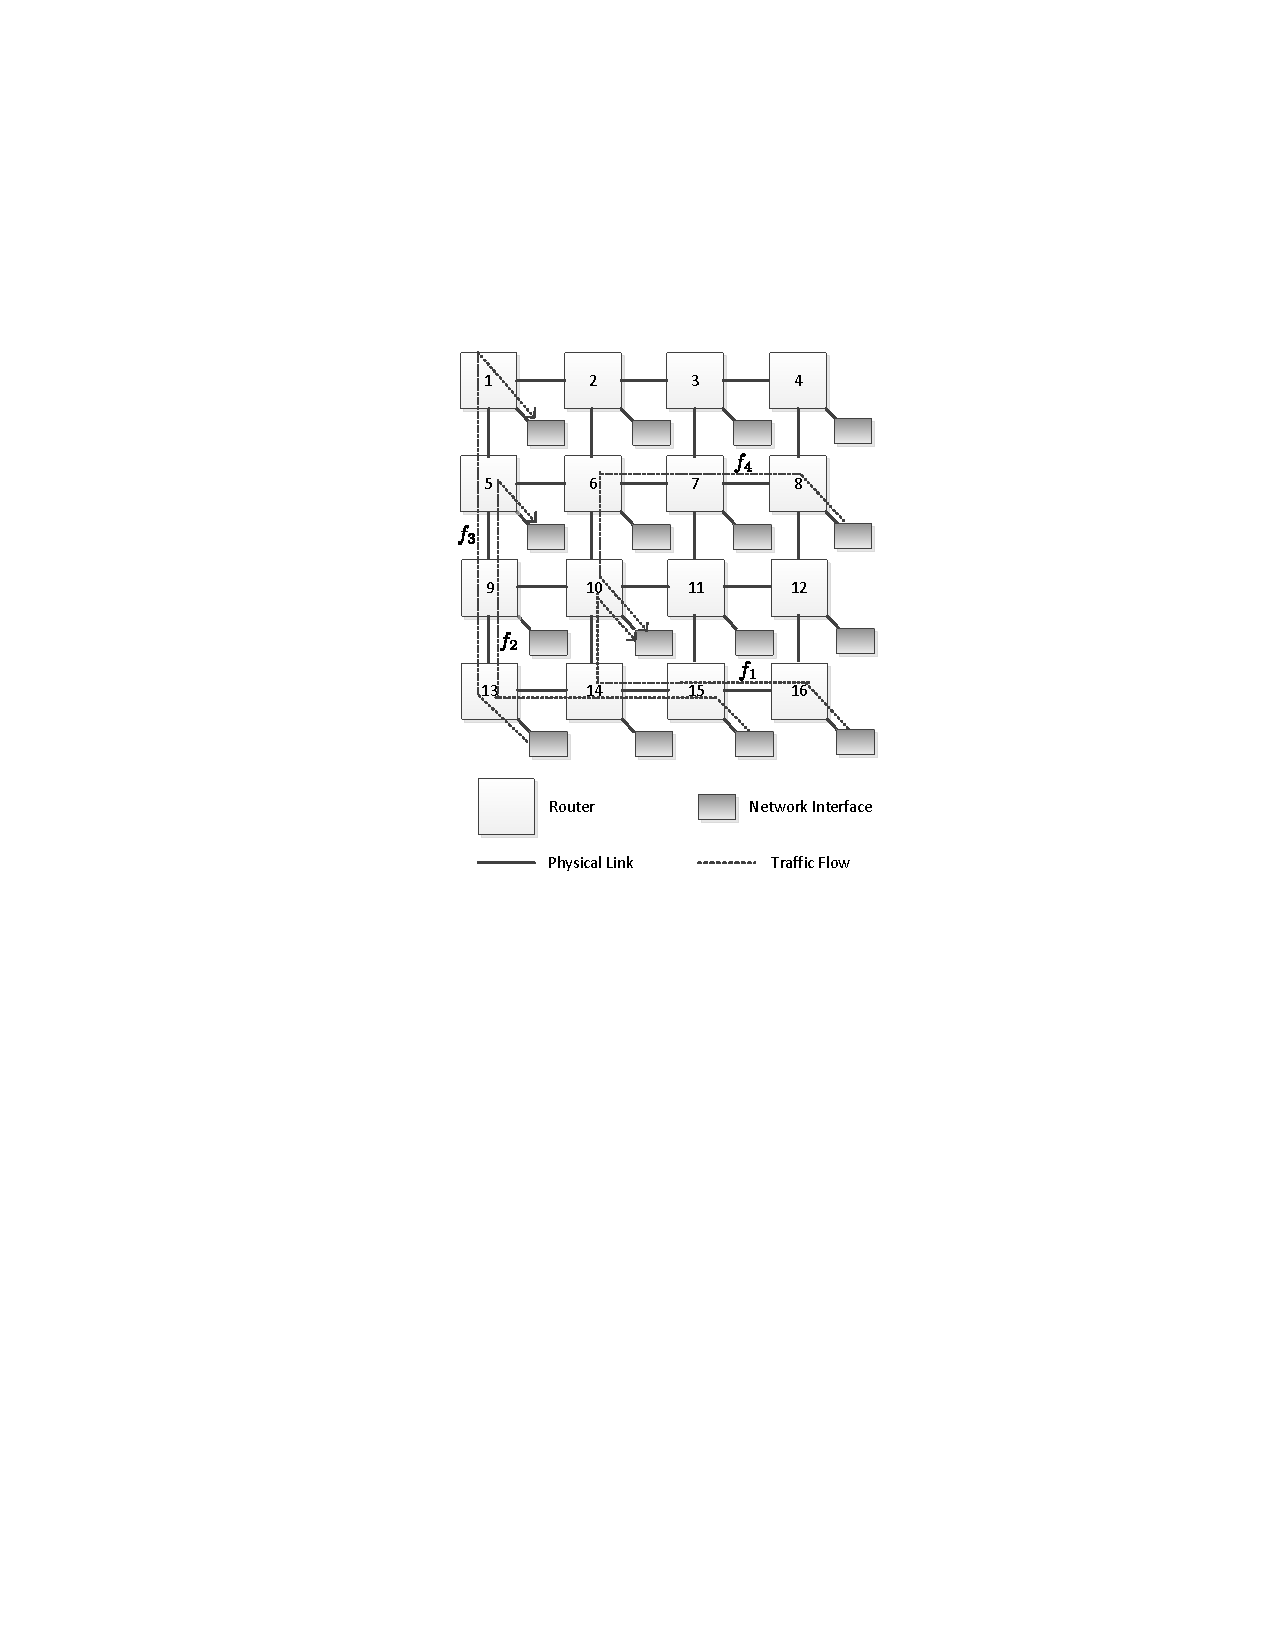
\includegraphics[scale=0.85]{fig1.pdf}
  \caption{Mesh topology with four real-time traffic flows.}\label{topology}
\end{figure}

Our performance model is topology-independent, but to demonstrate the basic idea, we take the mesh topology shown in Fig. \ref{topology} as an example throughout this paper. Routers in the mesh topology have five input/output ports, corresponding to the four cardinal directions (West, East, North and South) and the Local IP core. Although there are only four flows, i.e. $f_1$, $f_2$, $f_3$ and $f_4$, in the network, it is sufficient to demonstrate the idea of our method, and our method can handle more traffic flows efficiently. Our method extends the methods in \cite{Shi:2008:RCA:1397757.1397996}\cite{189}\cite{73} to allow multiple flows to share the same priority. But, to avoid deadlock and performance degradation caused by VC sharing, we assumes that each flow has a distinct VC at each router. Flits of different flows sharing the same priority are served in round-robin order when they compete the same output port. Since the minimum transmission unit in the priority-aware wormhole-switched NoC is flit and a high-priority flit can preempt the transmission of a low-priority flit, the router micro-architecture considered in this paper is flit-level preemptive \cite{Lee:2003:RWC:846077.846083}.

\subsection{Introduction to Real-Time Calculus}\label{intrortc}
Real-time calculus \cite{1253607} is the extension of the DNC theory \cite{Boudec2001Network}, by adding the upper service curve and lower arrival curve to describe the maximum service capability of a system and the minimum arrival rate of an event stream. Before introducing the concepts of the RTC arrival curve and service curve, we first present the symbols and operators used in this article, as listed in Table \ref{symbol}. Due to the space limitation, we only list the important properties used in this paper, as presented in Table \ref{properties}. For more details about DNC and RTC theory, please refer to \cite{Boudec2001Network}\cite{1253607}.
\begin{table}
  \centering
  \begin{tabular}{l|l}
    \hline\hline
    Symbols & Description \\
    \hline
    $\mathcal{N}$ & set of natural numbers\\
    $\lceil\cdot\rceil$ and $\lfloor\cdot\rfloor$ & ceiling operator and floor operator\\
    $1_{\{val\}}$ & indicator function, e.g. $1_{\{val\}}=1$ if and only if $val$ is true\\
    $\delta_{val}(t)$ & burst-delay function, e.g.  $\delta_{val}(t)=+\infty$ if $t>val$, else 0\\
    $\otimes$ & min-plus convolution, e.g. $f\otimes g=\min_{0\leq s\leq t}\{f(s)+g(t-s)\}$ \\
    $\oslash$ & min-plus de-convolution, e.g. $f\oslash g=\sup_{s\geq 0}\{f(t+s)-g(s)\}$ \\
    $\bar{\otimes}$ & max-plus convolution, e.g. $f\bar{\otimes} g=\sup_{0\leq s\leq t}\{f(t-s)+g(s)\}$ \\
    $\bar{\oslash}$ & max-plus de-convolution, e.g. $f\bar{\oslash} g=\inf_{s\geq 0}\{f(t+s)-g(s)\}$ \\
    $f^{(n)}$ & $n$th-fold min-plus convolution of $f$ and $f^{(0)}(t)=\delta_0(t)$\\
    $\bar{f}$ & sub-additive closure, e.g. $\bar{f}=\inf_{n\geq 0}\{f^{(n)}\}$\\
    $u_{T,\tau}$ & staircase function, e.g. $u_{T,\tau}=\lceil\frac{t+\tau}{T}\rceil$ if $t>0$, else 0\\
    \hline
  \end{tabular}
  \caption{Symbols and operators used in this article}\label{symbol}
\end{table}

\begin{rmk}[Real-Time Arrival Curve \cite{1253607}]\label{acu}
Denote by $R[s,t)$ the number of events within the time interval $[s,t)$. The lower and upper bounds on $R[s,t)$ are called the lower arrival curve $\alpha^l$ and upper arrival curve $\alpha^u$, which satisfy
$$\alpha^l(t-s)\leq R[s,t)\leq \alpha^u(t-s),\forall s<t$$
and $\alpha^l(0)=\alpha^u(0)=0$. The RTC arrival curve for a event stream is denoted as $<\alpha^l,\alpha^u>$ for short.
\end{rmk}

The above definition also provides a way to extract the RTC arrival curve from the synthetic traffic or communication trace, which is called sliding window method \cite{1253607}. For any time window $\Delta$, this method tries to find the maximal and minimal number of arrived flits (corresponding to $\alpha^l(\Delta)$ and $\alpha^u(\Delta)$) by analyzing the time series of flits.

\begin{rmk}[Real-Time Service Curve \cite{1253607}]\label{rtcsc1}
Denote by $S[s,t)$ the number of events that can be processed by the system in time interval $[s,t)$. The lower and upper bounds on $S[s,t)$ are called the lower service curve $\beta^l$ and upper service curve $\beta^u$, which satisfy
$$\beta^l(t-s)\leq S[s,t)\leq \beta^u(t-s),\forall s<t$$
and $\beta^l(0)=\beta^u(0)=0$. The RTC service curve for a system is denoted as $<\beta^l,\beta^u>$ for short.
\end{rmk}

From definition \ref{rtcsc}, we find that the sliding window method used to obtain the RTC arrival curve can also be utilized to get the RTC service curve, because the upper and lower service curve describe the maximum and minimum number of events processed by a system, respectively. Since these two concepts correspond to the service curve and maximum service curve in DNC theory \cite{Boudec2001Network}, we present the following equivalent definition of RTC service curve by combining the definition of service curve and maximum service curve in DNC theory \cite{Boudec2001Network}:

\begin{rmk}[Real-Time Service Curve \cite{Boudec2001Network}]\label{rtcsc2}
Denote by $R(t)$ and $R^*(t)$ the input and output function of a flow traversing server $\mathcal{S}$. We say that $\mathcal{S}$ offers to the flow an RTC service curve $<\beta^l,\beta^u>$ if and only if
$$R\otimes\beta^l(t)\leq R^*(t)\leq R\otimes \beta^u(t)$$
\end{rmk}

One of the most important theorem in RTC theory is the concatenation theorems for the lower service curve (see Theorem 1.46 in \cite{Boudec2001Network}) and upper service curve (see Theorem 1.6.1 in \cite{Boudec2001Network}). Assume an event stream traverses two systems $S_1$ and $S_2$ in sequence, and $S_i$ offers an RTC service curve $<\beta^l_i,\beta^u_i>$ $(i=1,2)$ to this event stream. The concatenation theorem can give the equivalent RTC service curve offered by these two systems to the event stream, which is $<\beta^l_1\otimes\beta^l_2,\beta^u_1\otimes\beta^u_2>$.

Other properties of network calculus theory used in this paper are listed in Table \ref{properties}.
\begin{table}
  \centering
  \begin{tabular}{l|l}
    \hline\hline
    Properties & Description \\
    \hline
    P1: Neutral element & $\forall f\in\mathcal{F}$, $f\otimes \delta_0=f$\\
    P2: Addition of a constant & $(f+K)\otimes g=f\otimes g+K$\\
    P3: Commutativity of $\otimes$ & $\forall f,g\in \mathcal{F}$, $f\otimes g=g\otimes f$\\
    P4: Associativity of $\otimes$ & $\forall f,g,h\in \mathcal{F}$, $(f\otimes g)\otimes h=f\otimes (g\otimes h)$\\
    P5: Closure of $\otimes$ & $f(0)=g(0)=0\Rightarrow \overline{f\otimes g}=\bar{f}\otimes\bar{g}$\\
    P6: Closure property & $\forall f\in\mathcal{F}$, $\bar{f}\otimes \bar{f}=\bar{f}$ and $\bar{\bar{f}}=\bar{f}$\\
    P7: Distribution with $\min$ & $\forall f,g,h\in \mathcal{F}$, $(\min\{f,g\})\otimes h=\min\{f\otimes h,g\otimes h\}$\\
    P8: Isotonicity of $\otimes$ & $\forall f,f^\prime,g,g^\prime\in \mathcal{F}$, $f\leq g$ and $f^\prime\leq g^\prime\Rightarrow f\otimes f^\prime\leq g\otimes g^\prime$\\
    \hline
  \end{tabular}
  \caption{Properties of min-plus convolution used in this article, where $K$ is non-negative real number and $\mathcal{F}$ is the set of wide-sense increasing functions such that $\forall f\in\mathcal{F}$, $f(t)=0$ for $t<0$.}\label{properties}
\end{table}

In this paper, we will utilize the discrete time RTC arrival curve and service curve to characterize the arrived traffic and service capability of the wormhole-switched NoC, since the minimum time unit of this system is the clock period $T$. Events in the definition \ref{acu} and \ref{rtcsc1} refer to the arrival and service of flits, respectively. If we obtain the arrival curve $<\alpha^l,\alpha^u>$ of a specific flow at specific router and the service curve $<\beta^l,\beta^u>$ provided by this router, we can get the output arrival curve $<\alpha^{l^\prime},\alpha^{u^\prime}>$ of this flow and leftover service curve $<\beta^{l^\prime},\beta^{u^\prime}>$ of this router with the following equations given in \cite{1253607}:
\begin{equation}\label{alphal}
\alpha^{l^\prime}=\min\{(\alpha^l\oslash\beta^u)\otimes\beta^l,\beta^l\}
\end{equation}
\begin{equation}\label{alphau}
\alpha^{u^\prime}=\min\{(\alpha^u\otimes\beta^u)\oslash\beta^l,\beta^u\}
\end{equation}
\begin{equation}\label{betal}
\beta^{l^\prime}=(\beta^l-\alpha^u)\bar{\otimes}0
\end{equation}
\begin{equation}\label{betau}
\beta^{u^\prime}=\max\{(\beta^u-\alpha^l)\bar{\oslash}0,0\}
\end{equation}

After obtaining the arrival curve $<\alpha^l_{f},\alpha^u_{f}>$ of flow $f$ and the equivalent service curve $<\beta_{f}^l,\beta_{f}^u>$ offered by the system to flow $f$, we can get the delay bound by the following equation \cite{Boudec2001Network}
\begin{equation}\label{delay}
Delay(f)=H(\alpha^u_{f},\beta^l_{f})
\end{equation}
where operator $H(\cdot,\cdot)$ computes the maximal horizontal deviation between its two operands.

\section{Delay Analysis and Buffer Sizing}\label{modeling}
In this section, we first build an RTC-based performance model for the priority-aware wormhole-switched NoC with credit-based flow control. Based on this performance model, we then propose an end-to-end delay analysis algorithm and a buffer sizing algorithm.

The performance model comprises two parts, i.e. traffic model and service model. The traffic model utilizes the RTC arrival curve to describe the arrival process of each flow. We will introduce a novel method to obtain the RTC arrival curve in subsection \ref{traffic}. The service model characterizes the services offered by the priority-aware NoC to each flow. The construction of the service model is much more complicated than the traffic model, and the following three issues should be considered: (1) Only the head flit needs to traverse the RC and VA stage of a router, because the non-head flits of a packet follow the data-path built by the head flit. To simplify our service model, we need a special mechanism to characterize the service offered to head and non-head flits in an unified way. (2) Our performance model supports priority sharing among flows. Thus, the computation of the leftover service curve provided to the lower-priority flows must be started after all the service curves of high-priority flows with Eq. \ref{betal} and Eq.\ref{betau} have been derived. (3) The cyclic-dependence between the adjacent routers caused by flow control makes the derivation of equivalent RTC service curve offered by the network very complex, which further prevents us from deriving the end-to-end delay bound with Eq.(\ref{delay}). Thus, we should first break this cyclic-dependence before analyzing the performance bound. We will discuss the first two issues in subsection \ref{sm}, and the last issue is discussed in subsection \ref{flowcontrol}. Then, we present two delay analysis algorithms in subsection \ref{e2elatency1} and subsection \ref{e2elatency2}, with each applying under different conditions.

Our router micro-architecture allows multiple flows sharing the same priority. But, to avoid deadlock and performance degradation, we assume that there exists an unique VC at each router for every distinct flows, which makes the implementation cost very expensive. To reduce the hardware overhead of this architecture, we propose a buffer sizing algorithm which allocates as small buffer space as possible to guarantee the deadline not be violated, as explained in subsection \ref{bufferopt}.

\subsection{Traffic Model}\label{traffic}
The communication in priority-aware wormhole-switched NoC is realized by transmitting packets, and each packet is divided into flits, which is the minimum transmission unit. Denote by $<\alpha^l(\Delta),\alpha^u(\Delta)>$ the flit arrival curve of a flow, namely, the minimum and maximum number of flits can be seen within any time window of length $\Delta$. We can extract the flit arrival curve from the synthetic traffic or communication trace with the sliding window method \cite{1253607}. For any time window $\Delta$, this method tries to find the maximal and minimal number of arrived flits (corresponding to $\alpha^l(\Delta)$ and $\alpha^u(\Delta)$) by analyzing the time series of flits. However, the obtained flit arrival curve can only be applied to compute the worst-case performance bound at the flit level, because the service model we constructed in the following subsection characterizes the services provided by the system at the flit level. To obtain the packet level delay bound, this arrival curve must be $L$-packetized \cite{Boudec2001Network}. Denote by $L(n)$ the cumulative packet length (in flits) of the first $n$ packets in a flow, $R(t)$ the cumulative arrived flits by time $t$. Then, the $L$-packetizer operator $\mathcal{P}^l(\cdot)$ is defined as $$\mathcal{P}^L(R(t))=\underset{n\in\mathcal{N}}{\sup}\{L(n)1_{L(n)\leq R(t)}\}.$$

Intuitively, $\mathcal{P}^l(R(t))$ can be interpreted as the largest cumulative packet length (in flits) contained in $R(t)$, as shown in Fig. \ref{lpkt}. Based on the definition of $\mathcal{P}^L(R(t))$ operator, we have
\begin{equation}\label{prop}
R(t)-l_{max}<\mathcal{P}^l(R(t))\leq \mathcal{R}(t)
\end{equation}
where $l_{max}$ is the maximum packet length (in flits).
\begin{figure*}
  \centering
  \subfloat[]{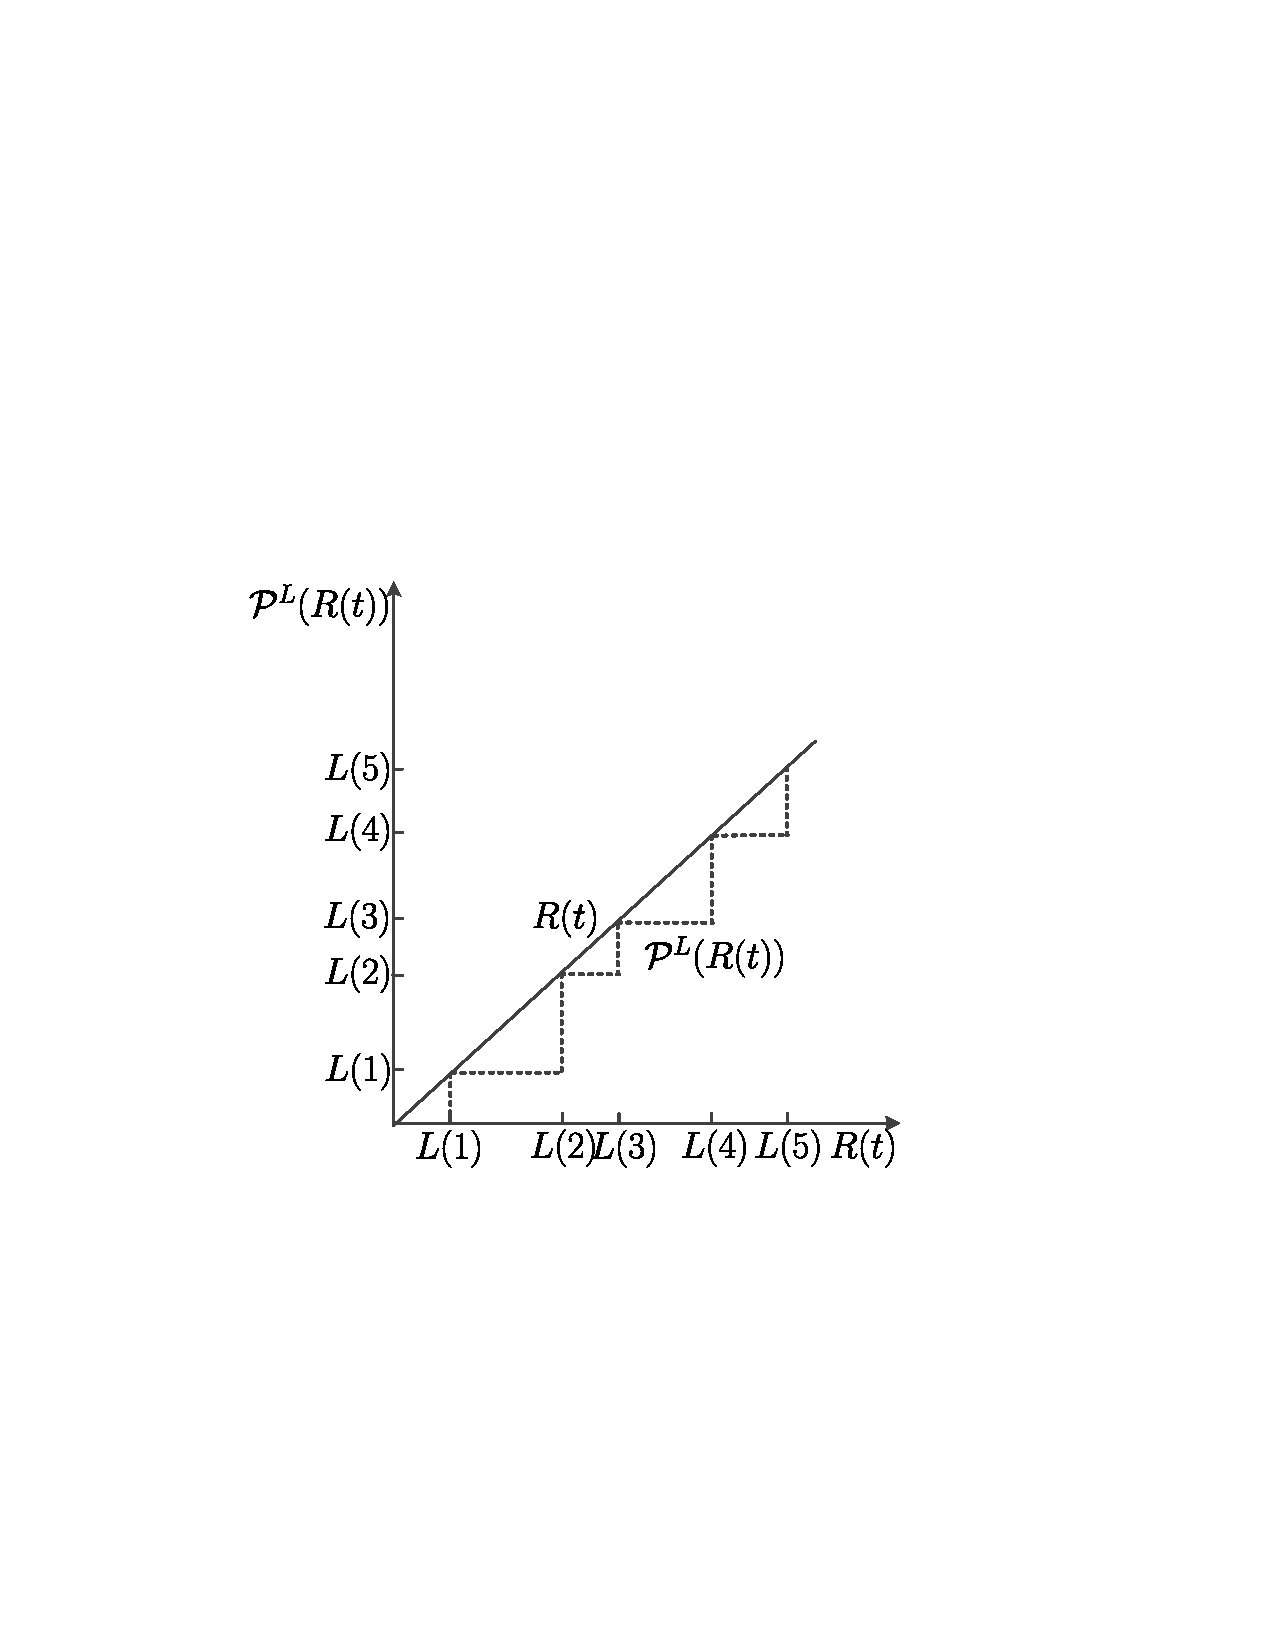
\includegraphics[scale=0.32]{fig2.pdf}\label{lpkt}}\hspace{10pt}
  \subfloat[]{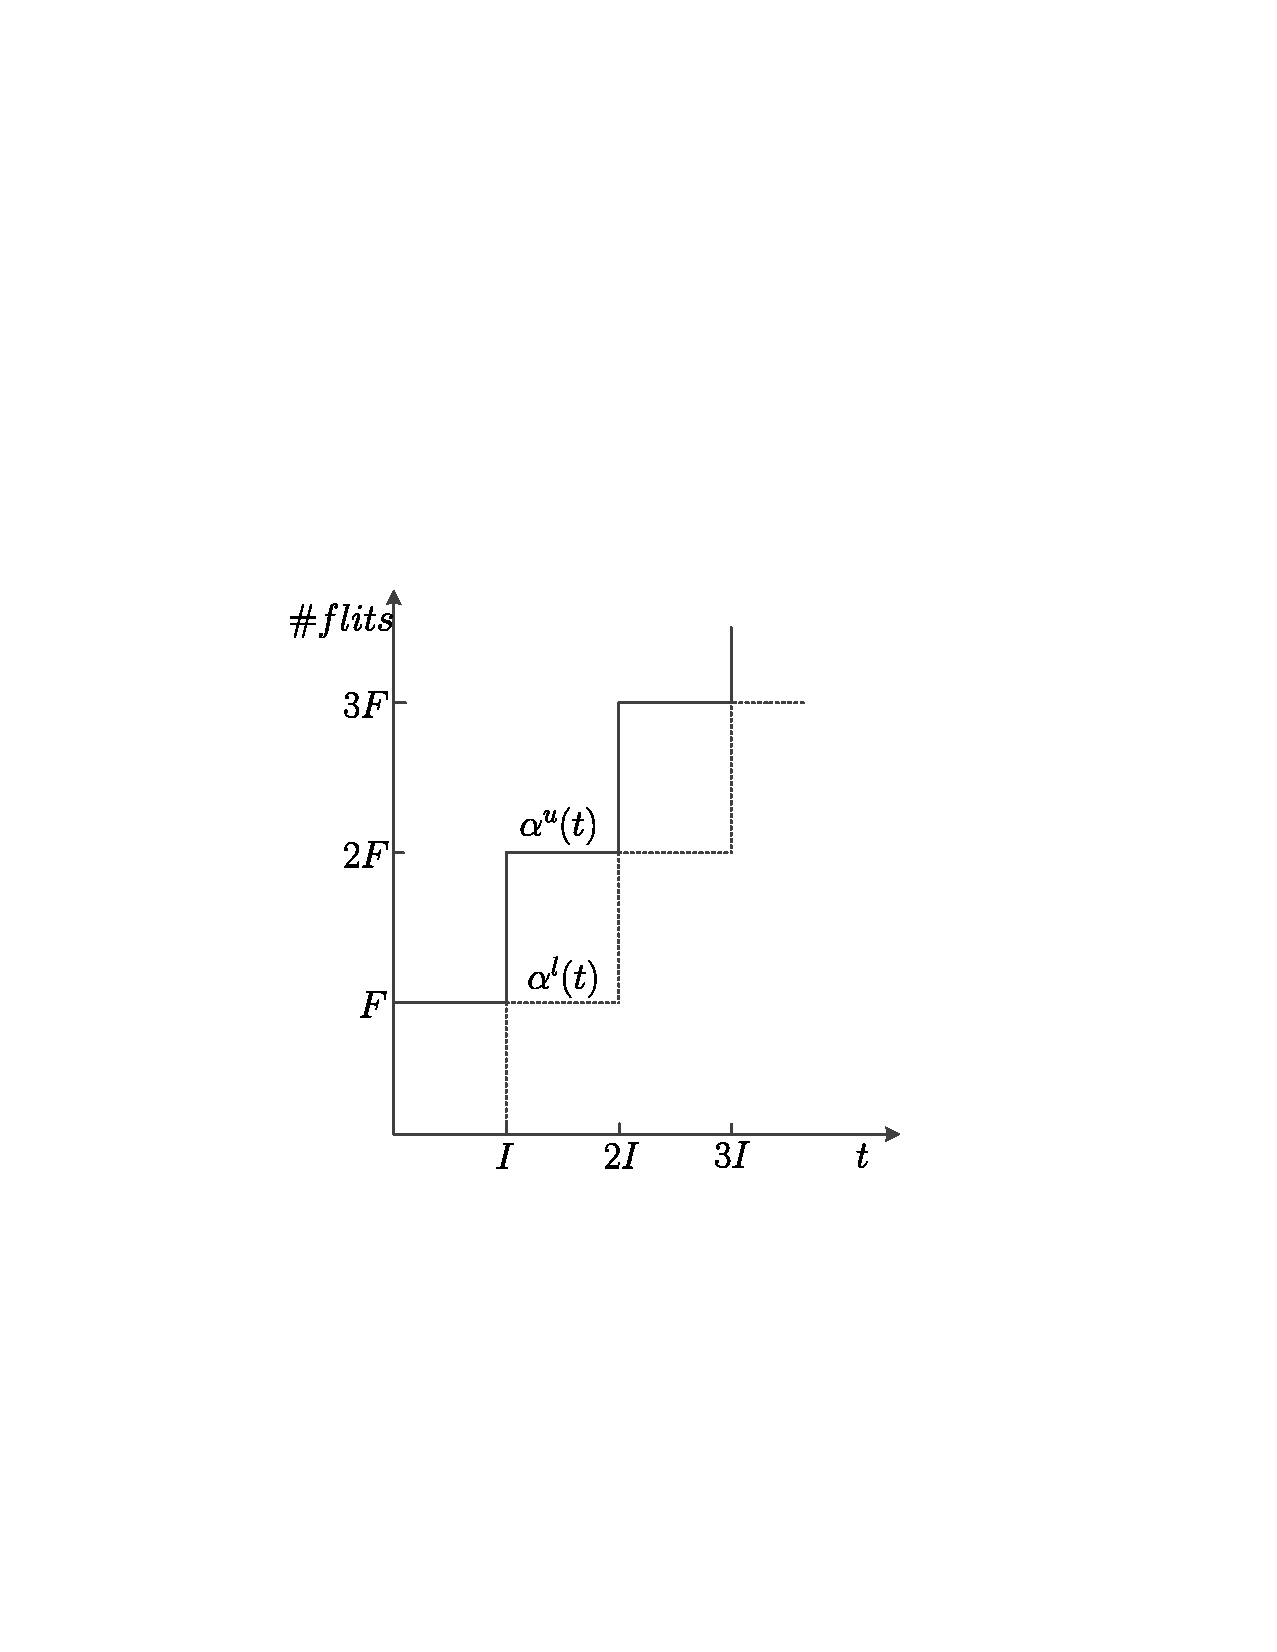
\includegraphics[scale=0.32]{fig3.pdf}\label{perio}}\hspace{10pt}
  \subfloat[]{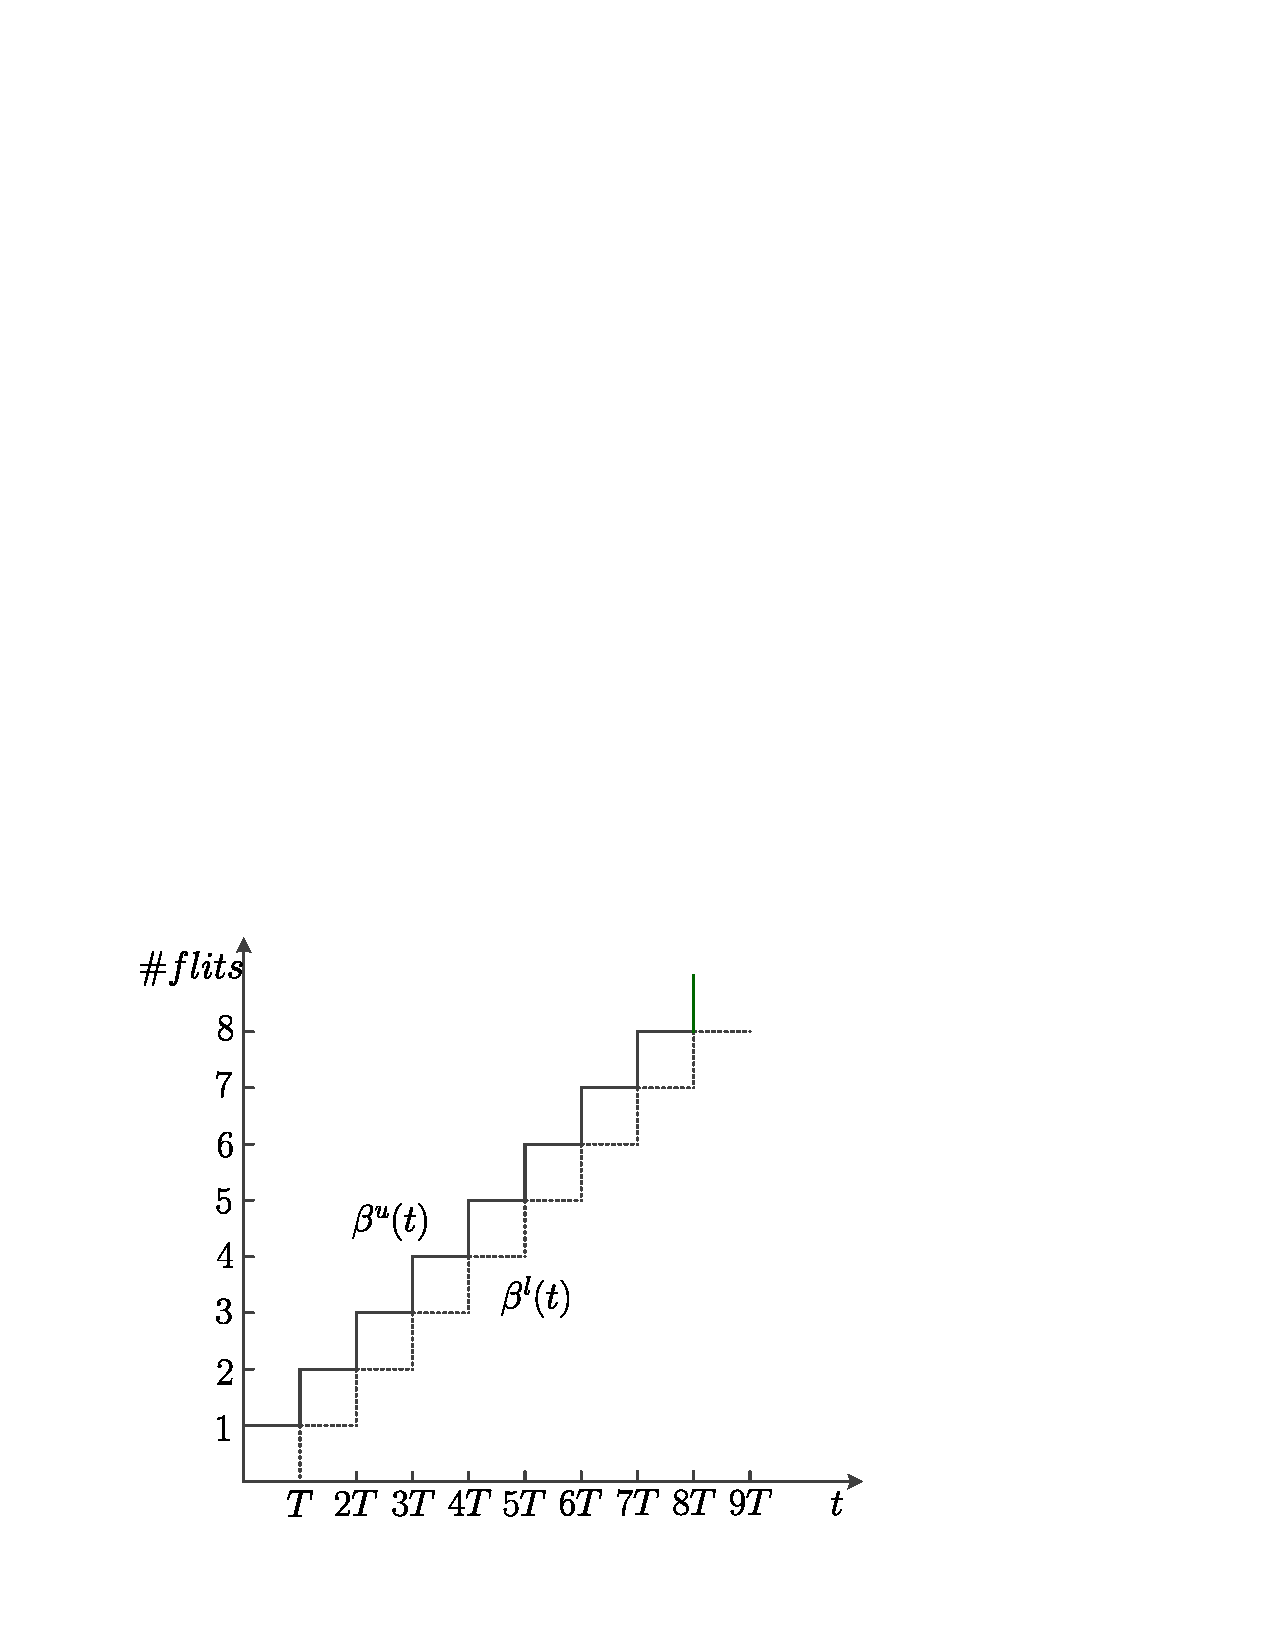
\includegraphics[scale=0.32]{fig4.pdf}\label{result1}}
  \caption{Traffic model and service model. (a) Definition of $\mathcal{P}^L(R(t))$. Cumulative arrival function $R(t)$ and the $L$-packetized cumulative arrival function $\mathcal{P}^L(R(t))$ are represented by the solid line and dotted line, respectively. (b) Real-time calculus arrival curve for periodically arrived traffic with period $I$ and packet length $F$. The solid line and dotted line represent the upper arrival curve and lower arrival curve. (c) Service model for each pipeline stage. The solid lines and dotted lines represent the upper service curves and lower service curves, respectively.}\label{ac}
\end{figure*}

In order to obtain the packet-level RTC arrival curve, we proposed the following theorem which transforms a flit-level RTC arrival curve to the $L-$packetized arrival curve.

\begin{thm}[$L$-packetized arrival curve]\label{pktac}
Suppose a flow has a flit arrival curve $<\alpha^l(\Delta),\alpha^u(\Delta)>$, and the maximum packet length (in flits) of this flow is $l_{max}$. Then, it has an $L$-packetized arrival curve $<\alpha^l(\Delta)-l_{max}1_{\{\Delta>0\}},\alpha^u(\Delta)+l_{max}1_{\{\Delta>0\}}>$.
\end{thm}
\begin{pf}
For $\forall t\geq 0,\Delta\geq 0$, according to Eq. (\ref{prop}), we have
$$R(t)-l_{max}< \mathcal{P}^L(R(t))\leq R(t)$$
and
$$R(t+\Delta)-l_{max}< \mathcal{P}^L(R(t+\Delta))\leq R(t+\Delta).$$

These two inequalities above indicate
$$R(t+\Delta)-R(t)-l_{max}< \mathcal{P}^L(R(t+\Delta))-\mathcal{P}^L(R(t))$$
and
$$\mathcal{P}^L(R(t+\Delta))-\mathcal{P}^L(R(t))< R(t+\Delta)-R(t)+l_{max}.$$

Based on the definition \ref{acu}, the $L$-packetized flow has a packet arrival curve $<\alpha^l(\Delta)-l_{max}1_{\{\Delta>0\}},\alpha^u(\Delta)+l_{max}1_{\{\Delta>0\}}>$, which ends the proof. \hspace*{\fill}~\QED\par\endtrivlist\unskip
\end{pf}

For some special cases, we can also obtain the $L$-packetized arrival curve directly instead of transformation from flit arrival curve. For example, suppose all the packets in a flow have the same length $F$ and arrived periodically with period $I$. By applying the sliding window method \cite{1253607}, we can obtain the flit arrival curve of this flow, which is a pair of staircase functions $<F\cdot u_{I,0},F\cdot u_{I,I}>$. As shown in Fig. \ref{perio}, the obtained flit arrival curve which is equal to the $L$-packetized arrival curve $\mathcal{P}^L(\alpha)$, since $\mathcal{P}^L(R(t))=R(t)$, $\mathcal{P}^L(\alpha^l(t))=\alpha^l(t)$ and $\mathcal{P}^L(\alpha^u(t))=\alpha^u(t)$.

\subsection{Feed-forward Service Model}\label{sm}
The service model characterizes the service obtained by each flow along its entire transmission path. The transmission path of a flow comprises of NI, routers and physical links. The service curve offered by a physical link can be obtained by applying the sliding window method \cite{1253607} which is a pair of staircase function $<u_{T,0},u_{T,T}>$ since it serves one flit per cycle. The service curves provided by the NI and routers will be discussed as follows.

\subsubsection{Service Curve Provided by Source NI}
Figure \ref{ni} illustrates the internal structure of this priority-aware NI, where the IP core can generate several flows simultaneously. Messages of different flows are encapsulated and stored in the dedicated buffer for that flow. The priority-aware scheduler selects one flit with the highest-priority at a time for transmission. Flits of different flows sharing the same priority are scheduled in round-robin order. Unscheduled flits will be imposed an additional latency $T$. A lower priority flow can transmit a flit if and only if there are no contending flits from higher priority or the high priority flits are blocked due to flow control. The RTC service curve provided by the source NI (denoted as $<\beta^l_{NI},\beta^u_{NI}>$) to all these flows can be obtained by applying the sliding window method \cite{1253607}, which is a pair of staircase functions $<u_{T,0},u_{T,T}>$, as shown in Fig. \ref{result1}.
\begin{figure}
  \centering
  % Requires \usepackage{graphicx}
  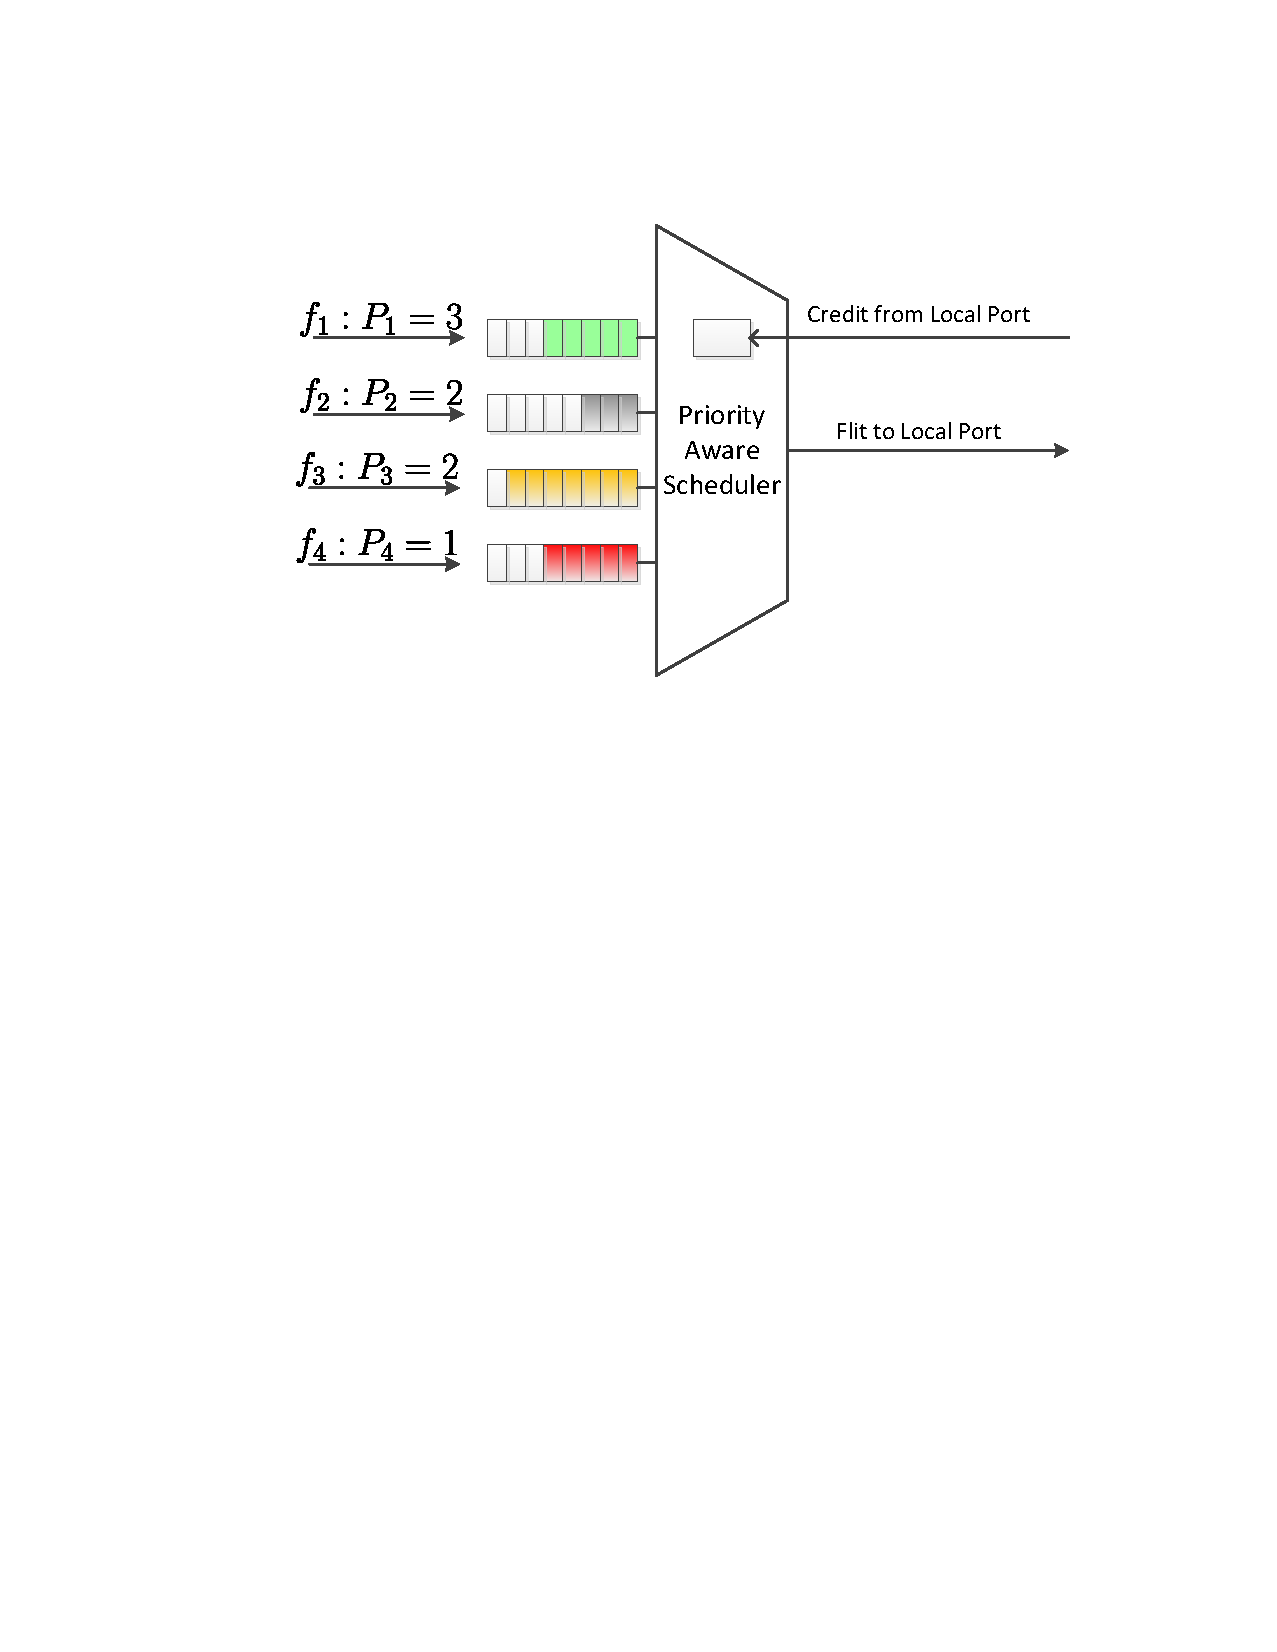
\includegraphics[scale=0.45]{fig5.pdf}
  \caption{Structure of priority-aware network interface. Each flow has its dedicated buffer, and the scheduler schedules the flit with the highest-priority to go through the output link at each cycle. Flows with the same priority are scheduled in Round-Robin order.}\label{ni}
\end{figure}

Given the set of flow specifications, the RTC service curve obtained by each flow at the source NI can be derived by applying Algorithm \ref{alg:scatni}. The flow specification of $f_j$ is a quadruple $(<\alpha^l_{f_j},\alpha^u_{f_j}>,\mathcal{R}_j,D_j,P_j)$ which specifies the RTC arrival curve, routine, deadline and priority.
\begin{algorithm}
\caption{Compute the service curve at source NI}\label{alg:scatni}
\begin{algorithmic}[1]
\Require $(<\alpha^l_{f_j},\alpha^u_{f_j}>,\mathcal{R}_j,D_j,P_j)$ // the set of flow specifications
\Ensure $<\beta_{NI,f_j}^l,\beta_{NI,f_j}^u>$ // the RTC service curve obtained by flow $f_j$
\State Group the flows with priority $P_i$ into subset $\mathcal{F}_i$.
\State $\beta_{NI}^{l^\prime}=\lfloor\frac{t}{T}\rfloor$; $\beta_{NI}^{u^\prime}=\lceil\frac{t}{T}\rceil$.
\For {each $\mathcal{F}_i$ from highest priority to lowest priority}
    \For {each flow $f_j\in \mathcal{F}_i$}
        \State $\beta_{NI,f_j}^l=\lfloor\frac{\beta_{NI}^{l^\prime}}{|\mathcal{F}_i|}\rfloor$; //$|\mathcal{F}_i|$ denotes the cardinality of $\mathcal{F}_i$
        \State $\beta_{NI,f_j}^u=\lceil\frac{\beta_{NI}^{u^\prime}}{|\mathcal{F}_i|}\rceil$.
    \EndFor
    \State $\alpha^l=\sum_{f_j\in \mathcal{F}_i}\alpha^l_{f_j}$; $\alpha^u=\sum_{f_j\in \mathcal{F}_i}\alpha^u_{f_j}$;
    \State $\beta_{NI}^{l^\prime}=(\beta_{NI}^{l^\prime}-\alpha^u)\bar{\otimes}0$; $\beta_{NI}^{u^\prime}=\max\{(\beta_{NI}^{u^\prime}-\alpha^l)\bar{\oslash}0,0\}$.
\EndFor
\end{algorithmic}
\end{algorithm}

\subsubsection{Basic Feed-Forward Service Curve Provided by Routers}\label{router}
While modeling the service capability of a router with RTC, we can analyze the data-path of a flow in the router stage-by-stage. Once we obtain the service curves offered by each stage, the service curve provided by the router to a flow can be derived by concatenating all these service curves. This is significantly different from the existing DNC based model \cite{qian2009analysis,Qian489900}, where they treat the entire router as a whole and designate a Latency-Rate (LR) service curve \cite{Boudec2001Network} to simplify the performance bounds derivation. Whereas, our model uses the staircase functions to characterize the detailed behavior of this discrete time system. The advantage of our method is that, it can be easily modified to characterize the non-standard router micro-architectures, by simply letting the service curve of non-existed stages to be a burst-delay function $\delta_0(t)$. Next, we try to derive the service curves of all these stages:

(1) BW stage, SA stage and LT stage: all the flits within a traffic flow will go through these three stages, and experience a fixed delay $T$ at each stage. The service curves provided by these stages, i.e. $<\beta^l_{BW},\beta^u_{BW}>$, $<\beta^l_{SA},\beta^u_{SA}>$ and $<\beta^l_{LT},\beta^u_{LT}>$, can be derived by applying the sliding window method \cite{1253607}, which are the same as the service curve of source NI, as shown in Fig. \ref{result1}.

(2) RC stage and VA stage: the latency of head flit experienced at these two stages is T. Although the non-head flits do not go through these two stages, they have to wait for at most two cycles before entering the SA stage at the worst-case when they are written into buffer consecutively after the head flit, e.g. the first three body flits of a packet shown in Fig. \ref{pipeline}. Thus, a sophisticated solution to construct a unified lower service curve for head flit and non-head flits at these two stages comes from viewing each of these two stages impose an additional delay $T$ for all the non-head flits. Thus, the equivalent lower service curve of these two stages, i.e. $\beta^l_{RC}$ and $\beta^l_{VA}$, can be obtained by applying the sliding window method \cite{1253607}, which are equal to the staircase function $u_{T,0}(t)$. To derive the upper service curve of these two stages, let us consider the best-case scenario, e.g. the tail flit shown in Fig. \ref{pipeline}. This delayed flit may be blocked by flow control or preempted by higher priority flits at upstream router. But, it can enter the SA stage immediately after it was written into the dedicated VC buffer because all the other flits have passed this stage. For this case, the RC and VA stages impose a zero latency to this flit. Thus, we can utilize the burst-delay function $\delta_0(t)$ to represent the upper service curve of these two stages.
\begin{figure}
  \centering
  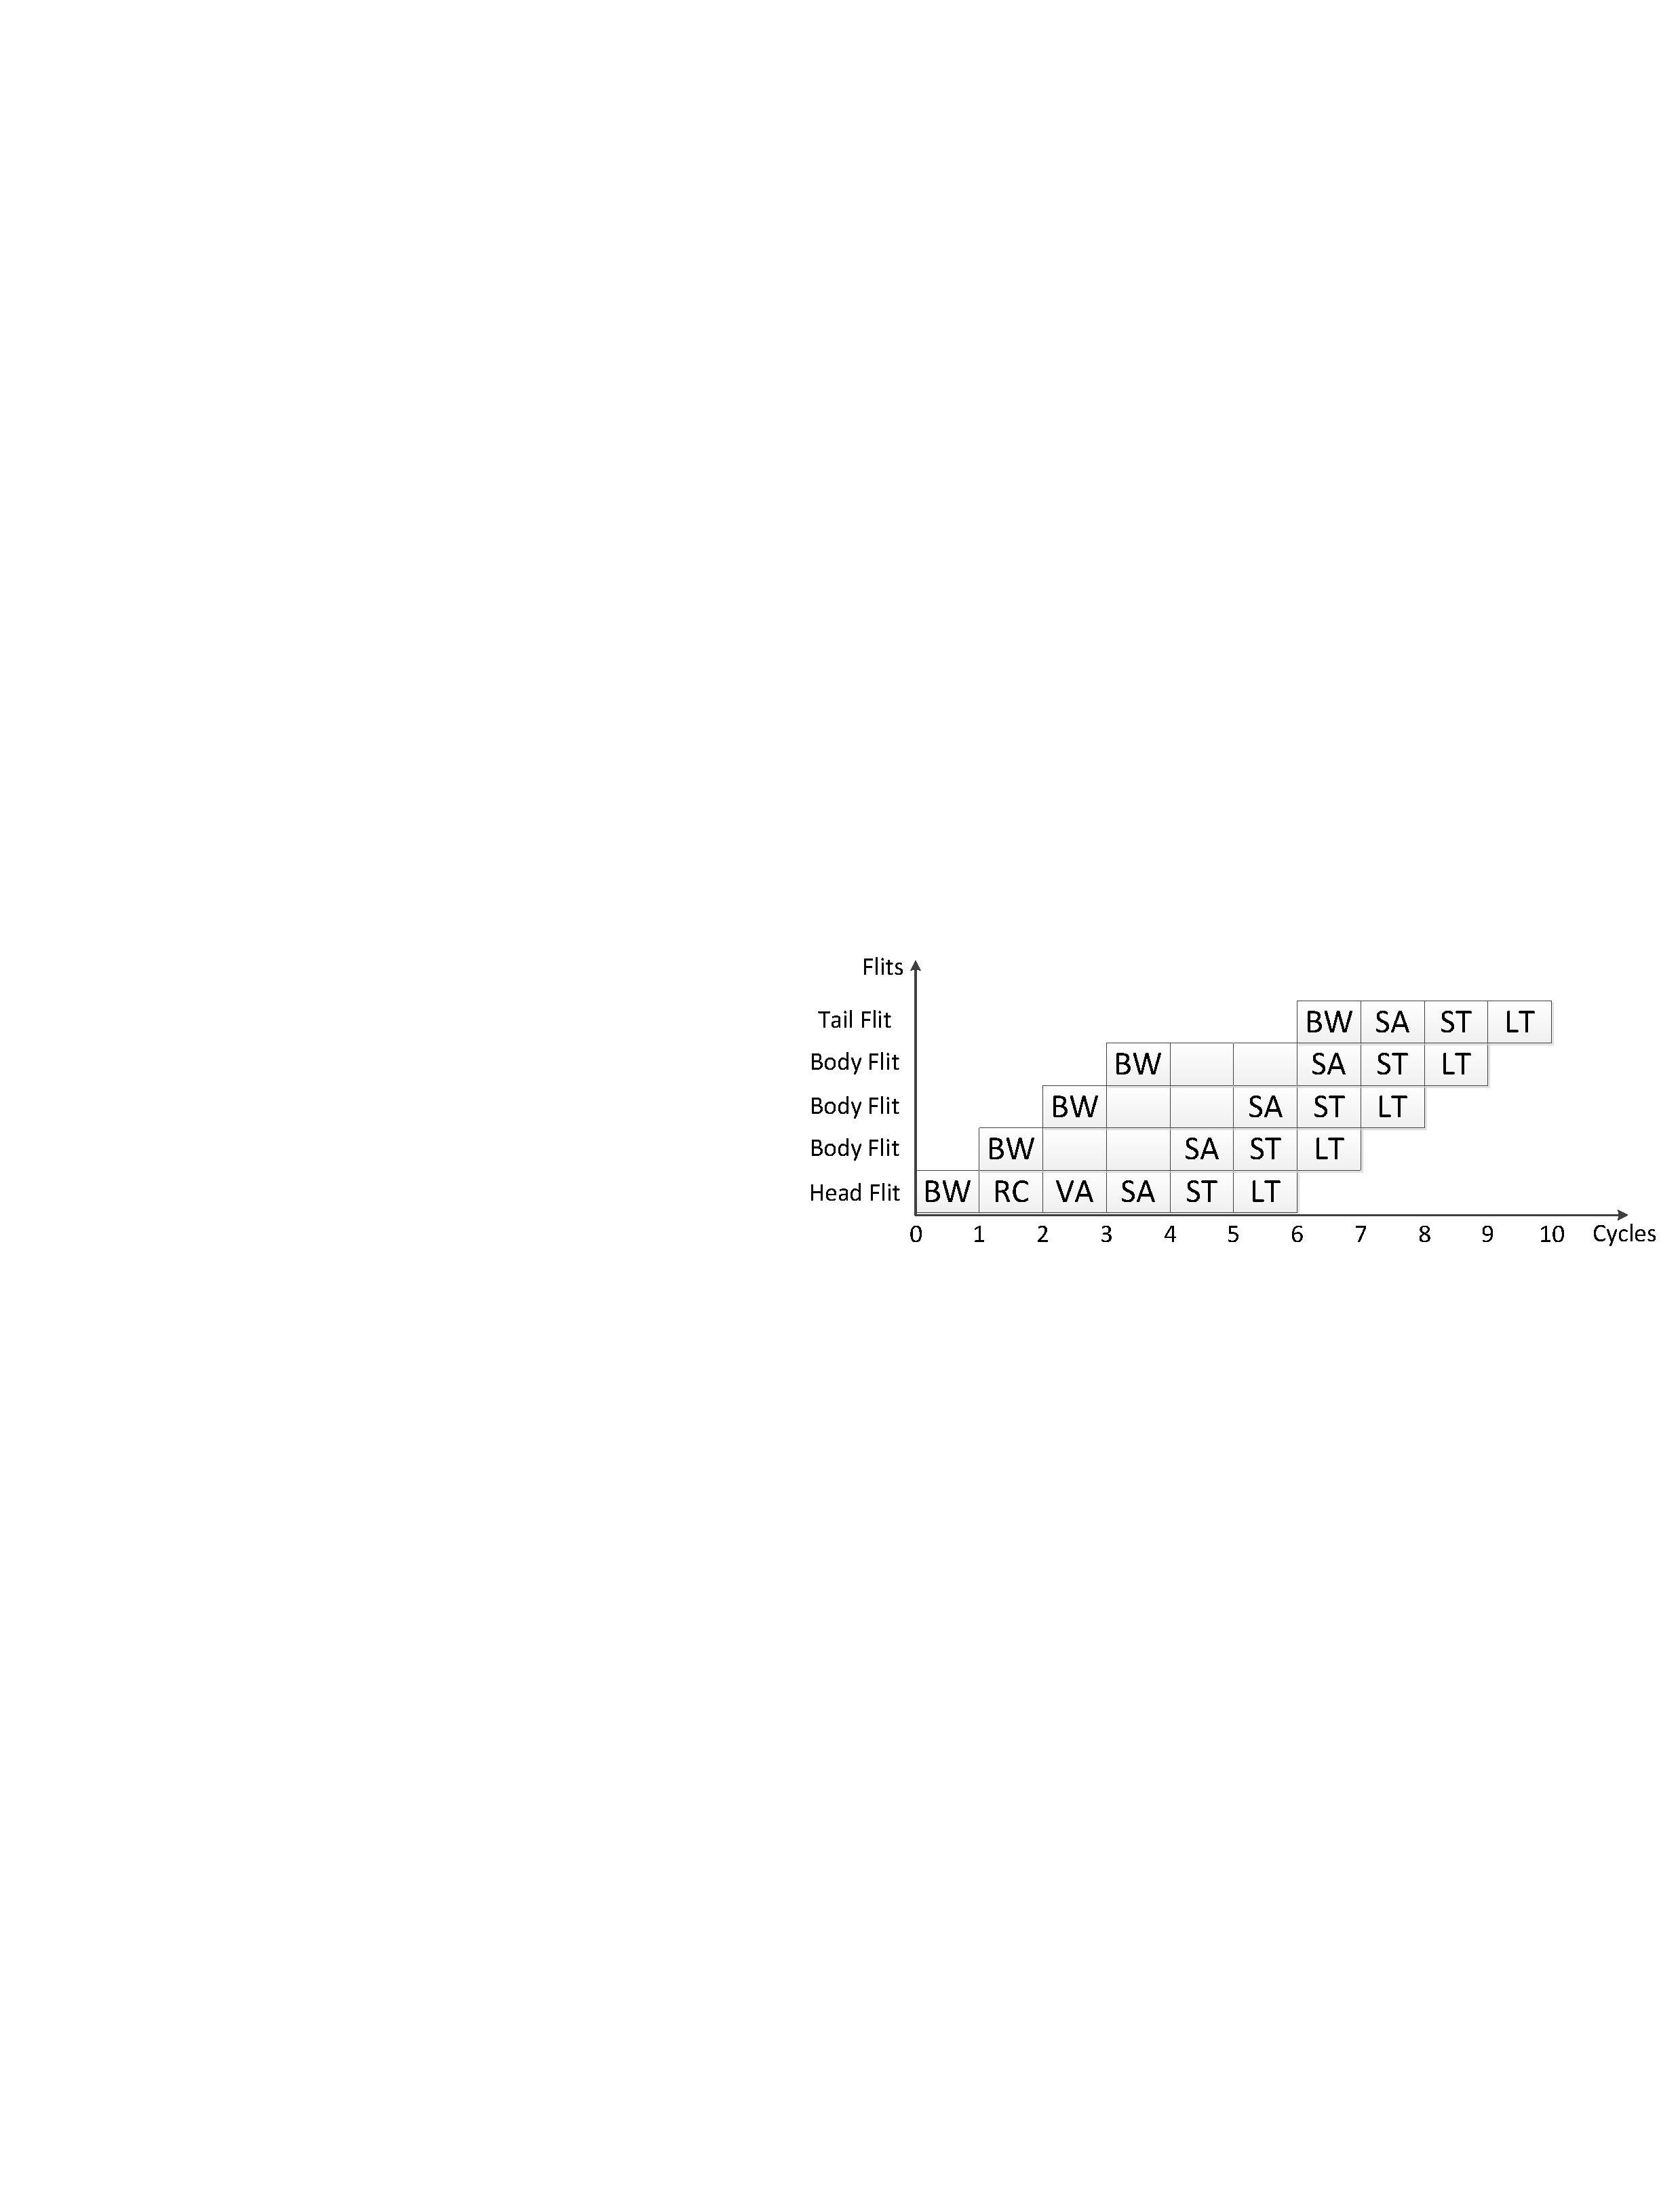
\includegraphics[scale=0.35]{fig6.pdf}
  \caption{Time-line graph of a packet going through the standard router pipeline. The delayed tail flit enters the ST stage immediately after it is written into the dedicated buffer.}\label{pipeline}
\end{figure}

(3) ST stage: each output port of the wormhole-switched NoC has a switch allocator to schedule the switch traversal among all the contending flows at each clock cycle. Denote by $<\beta_{ST,R_i^{p}}^l,\beta_{ST,R_i^{p}}^u>$ the total service provided by the ST stage to all the contending flows targeting to output port $p$. For the mesh topology, let the port indicator $p$ be $W$ (West port), $E$ (East port), $S$ (South port), $N$ (North port) or $L$ (Local port). Thus, Following the same procedure as BW stage, we can get $<\beta_{ST,R_i^{p}}^l,\beta_{ST,R_i^{p}}^u>$, which is $<u_{0,T}(t),u_{T,T}(t)>$, as shown in Fig. \ref{result1}.

It can be found that the contention of different flows within a router only might occur at ST stage. For the fixed-priority scheduling policy, switch allocators schedule the flow with the highest priority first, flows with the same priority will be served with round-robin order. All the unscheduled flows will impose an additional latency $T$ due to the failure of switch arbitration.

Denote by $<\beta_{ST,R_i,f_j}^l,\beta_{ST,R_i,f_j}^u>$ the service curve provided to flow $f_j$ by ST stage of router $R_i$, and $<\beta_{ST,R_i^{p}}^{l^\prime},\beta_{ST,R_i^{p}}^{u^\prime}>$ the leftover service curve after serving all the flows with higher priority than $f_j$. In order to obtain the service curve $<\beta_{ST,R_i,f_j}^l,\beta_{ST,R_i,f_j}^u>$, we should consider the following two cases:

(a) All the flows contending with $f_j$ at $R_i$ have lower priorities than $f_j$. For the synchronized router architecture, flow $f_j$ gets the total service curve $<\beta_{ST,R_i^{p}}^{l^\prime},\beta_{ST,R_i^{p}}^{u^\prime}>$.

(b) There exist some contention flows with the same priority as $f_j$. Since $f_j$ and all the flows in $\Theta_{R_i,f_j}$ got serviced in round-robin order, the service curve provided to $f_j$ is $<\lfloor\beta^{l^\prime}_{ST,R_i^{p}}/(|\Theta_{R_i,f_j}|+1)\rfloor,\lceil\beta^{u^\prime}_{ST,R_i^{p}}/(|\Theta_{R_i,f_j}|+1)\rceil>$ where operator $|g|$ represents the cardinality of set $g$. After serving all the flows in $\Theta_{R_i,f_j}$, the leftover service curve for low-priority flows can be derived by applying Eq.(\ref{betal}) and Eq.(\ref{betau}).

After we obtained the service curve provided by the ST stage of router $R_i$ to flow $f_j$, we can get the equivalent feed-forward service curve of router $R_i$ provided to $f_j$, i.e. $<\beta_{R_i,f_j}^l,\beta_{R_i,f_j}^u>$, by concatenating the service curves of all these stages together:
$$\beta_{R_i,f_j}^l=\beta_{BW}^l\otimes\beta_{RC}^l\otimes\beta_{VA}^l\otimes\beta_{SA}^l\otimes \beta_{ST,R_i,f_j}^l,$$
$$\beta_{R_i,f_j}^u=\beta_{BW}^u\otimes\beta_{RC}^u\otimes\beta_{VA}^u\otimes\beta_{SA}^u\otimes \beta_{ST,R_i,f_j}^u.$$

\subsection{Feedback Service Model}\label{flowcontrol}
To this end, we have constructed the traffic model and the basic feed-forward service model. However, the basic service model is only able to characterize the wormhole-switched NoC without credit-based flow control. Flow control introduces cyclic-dependence between the adjacent routers, and blocks a flow when there is no buffer space available at the downstream router. The cyclic-dependence between the adjacent routers prevents us from deriving the performance bound directly even after we have obtained the service curve reserved at each router for the target flow.

In existing literature, this problem is addressed by fixed-point iteration \cite{schioler2005network} or transformation from marked dataflow graph \cite{Thiele:2009:MPA:1629335.1629353}. In this subsection, we will try to tackle the same problem with another solution. Our new solution is inspired by \cite{qian2009analysis}, in which the authors abstract the flow control as a network element (called flow controller) providing an DNC service curve, and this service curve can be obtained by applying some basic properties of DNC theory \cite{Boudec2001Network}. To make the discussion concrete, we take flow $f_2$ in Fig. \ref{topology} as an example and utilize the scheduling network model \cite{1253607} to visualize the credit-based flow control. The complex relationship among $f_2$ and the other flows are shown in Fig. \ref{f2}. For brevity and clarity, we ignore flow $f_4$ and the flow control of the other flows in this figure. We also assume that, all the destination IP cores can consume the arrived flits immediately, thus there is no flow control between the ejection router and destination NI. However, to prevent the buffer overflow, the flow control between source NI and injection router is necessary.
\begin{figure*}
  \centering
  % Requires \usepackage{graphicx}
  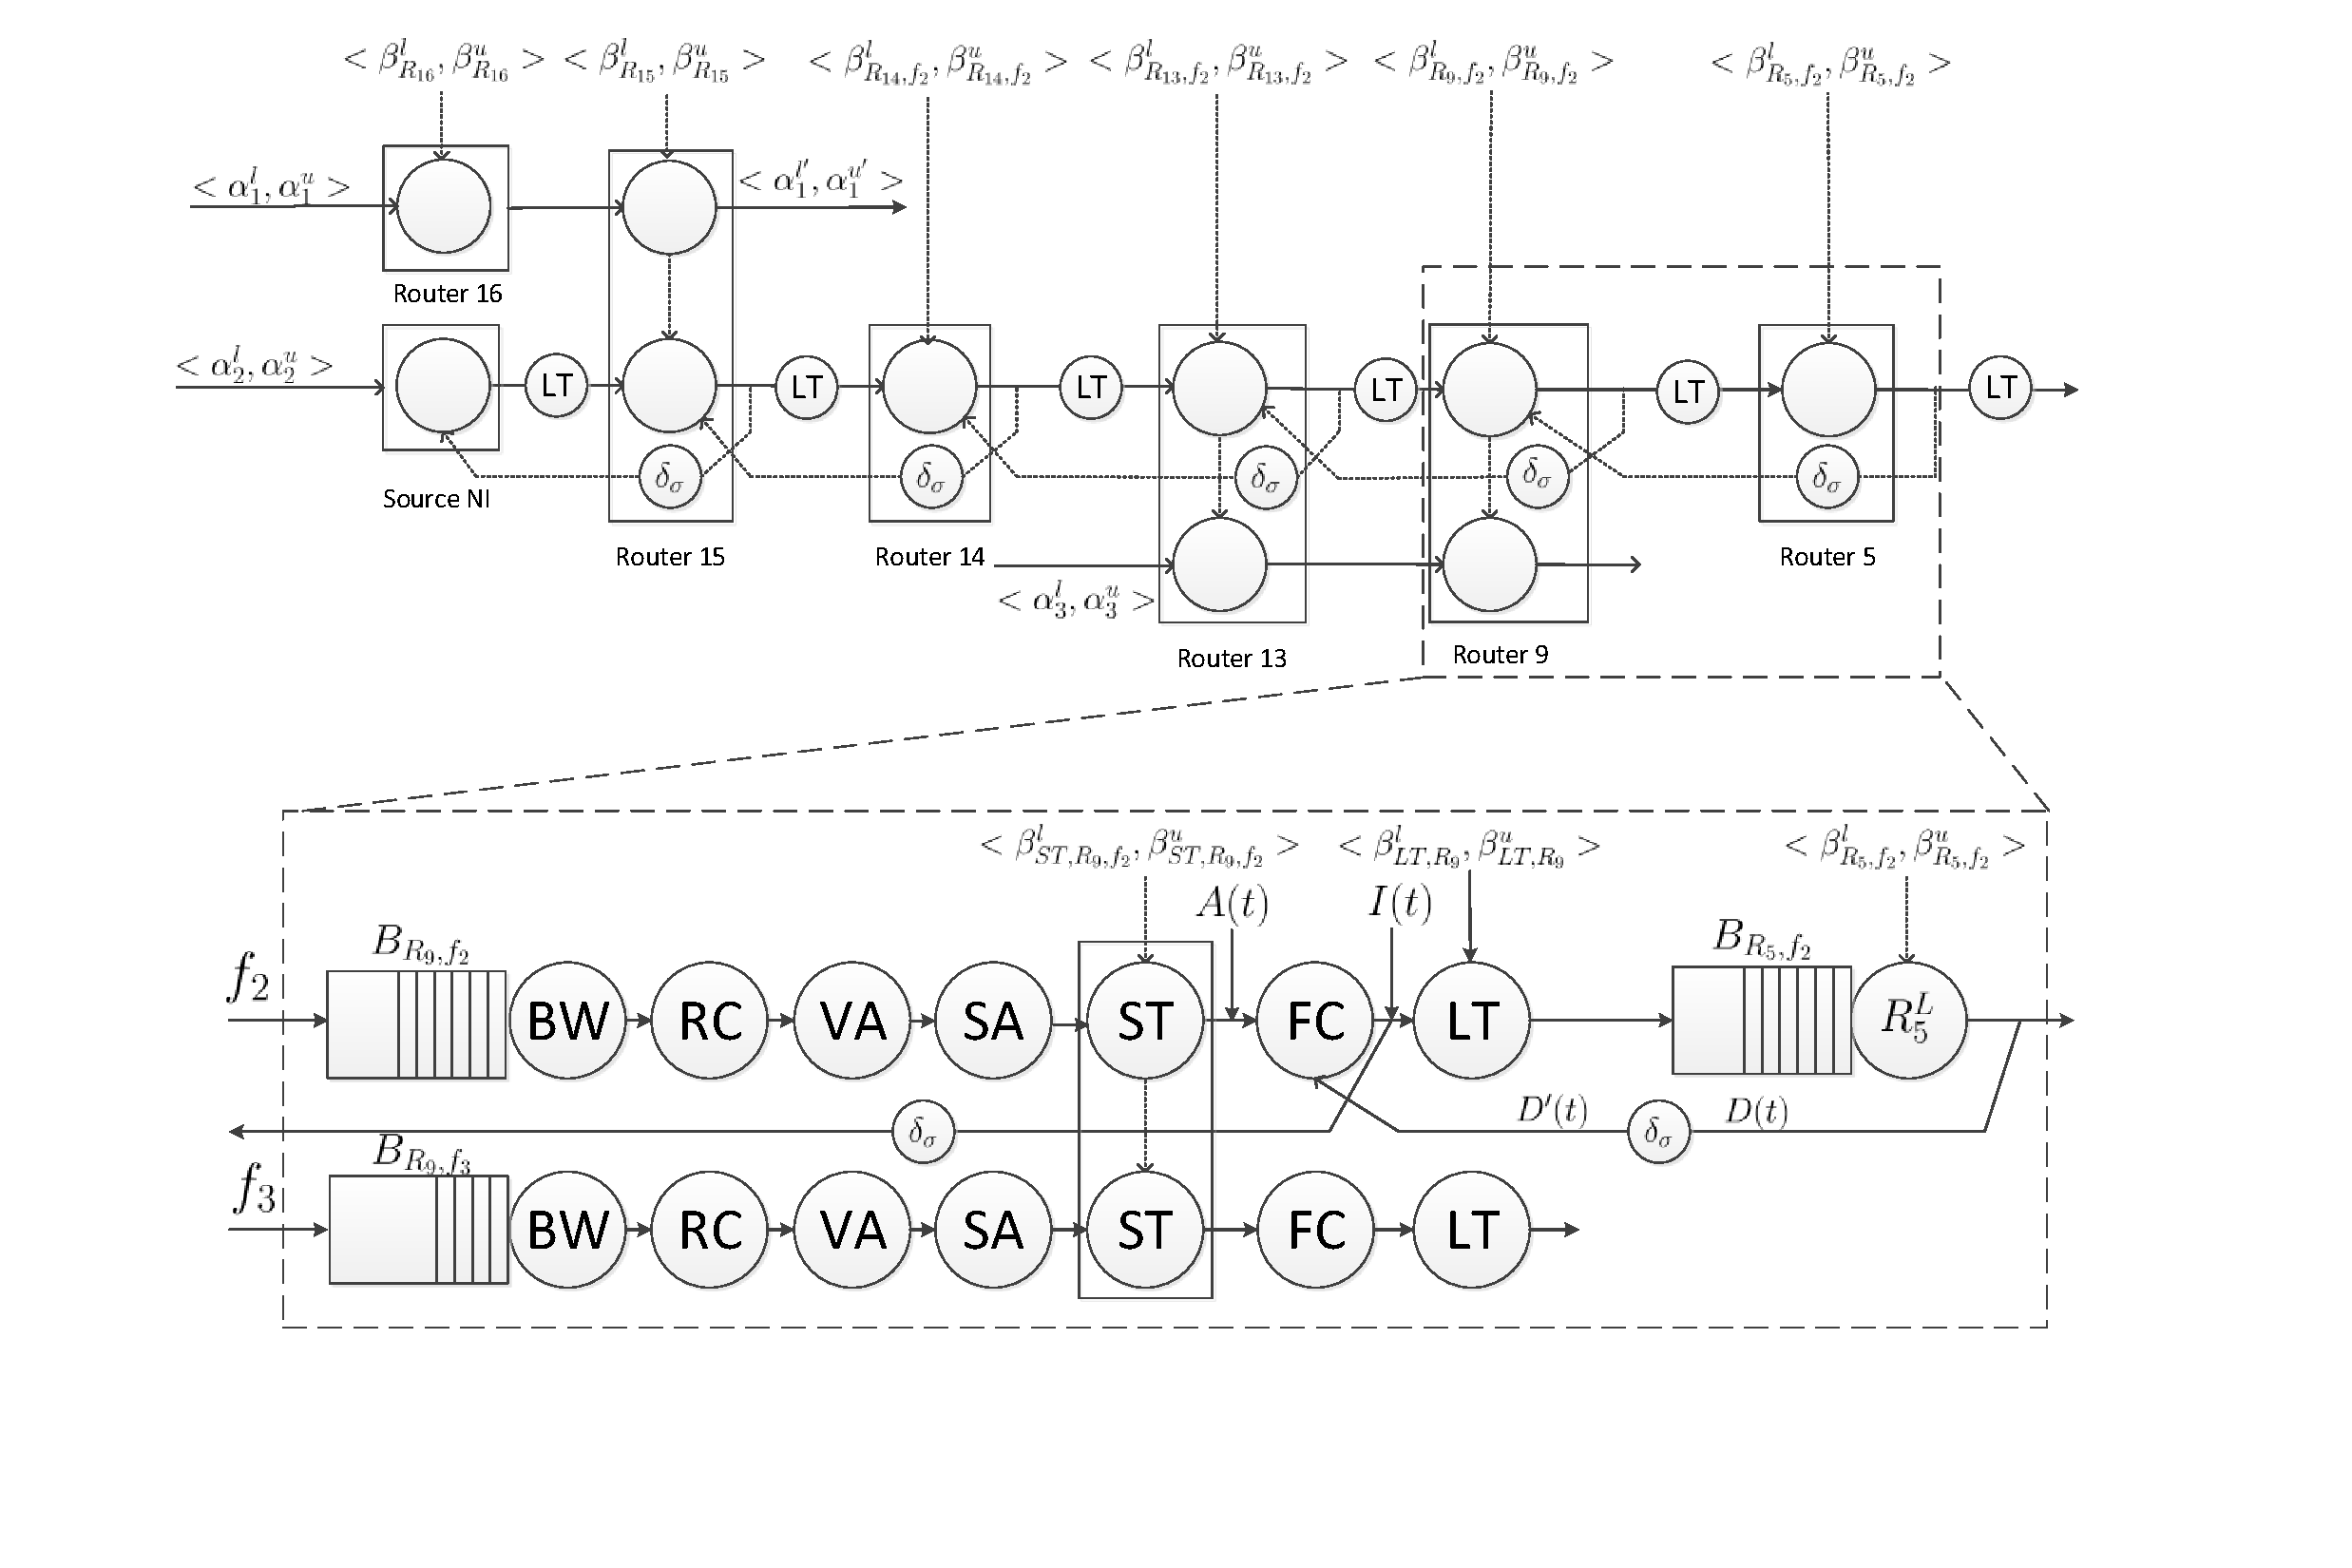
\includegraphics[scale=0.35]{fig7.pdf}\\
  \caption{Scheduling network model for flow $f_2$}\label{f2}
\end{figure*}

A flow in the wormhole-switched router with credit-based flow control will be blocked if there is no credit available. We can treat the flow controller as a virtual pipeline stage of a router, called Flow Control (FC) stage, as shown in Fig. \ref{f2}. The service curve of FC stage can be obtained by the following theorem. This theorem enables us to break the cyclic-dependence caused by flow control and obtain an equivalent feed-forward RTC service curve for the wormhole-switched router.
\begin{thm}\label{credit}
Suppose that a router provides a feed-forward service curve $<\beta^l,\beta^u>$, and the physical link provides service curve $<\beta_{LT}^l,\beta_{LT}^u>$, the buffer size and credit feedback delay are denoted as $B$ and $\sigma$, respectively. Then, the corresponding FC stage provides an RTC service curve $<\overline{\beta^l\otimes\beta_{LT}^l\otimes\delta_{\sigma}+B},\overline{\beta^u\otimes\beta_{LT}^u\otimes\delta_{\sigma}+B}>$.
\end{thm}
\begin{pf}
We will take the flow controller between $R_9$ and $R_5$ in Fig. \ref{f2} as an example to derive the service curve of flow controller. As has been proved in \cite{qian2009analysis}, the flow controller of $R_9$ provides an DNC service curve (i.e. RTC lower service curve) $\overline{\beta^l_{R_5,f_2}\otimes\beta_{LT}^l\otimes\delta_{\sigma}+B_{R_5,f_2}}$.

In the rest of this proof, we will derive the upper service curve for the flow controller. Denote the amount of injected and departed flits at $R_5$ by time $t$ as $I(t)$ and $D(t)$, and the amount of flits served by $R_9$ by time $t$ as $A(t)$. The feedback link can be represented as a network element providing upper service curve $\delta_\sigma(t)$. For the flow control between router $R_9$ and $R_5$, we have $I(t)\leq A(t)$ for causality and $I(t)\leq D^\prime(t)+B_{R_5,f_2}$ due to the effect of flow control, where $D^\prime(t)\leq D\otimes\delta_\sigma(t)$. Thus, $$I(t)\leq\min\{A(t),D^\prime(t)+B_{R_5,f_2}\}.$$

Based on the equivalent definition of upper service curve (i.e. definition \ref{rtcsc2}), we have $$D(t)\leq I\otimes \beta_{LT}^u(t)\otimes\beta_{R_5,f_2}^u.$$

Bring $I(t)$ and $D^\prime(t)$ into the above inequality, we get
\begin{eqnarray*}
D(t)&\leq& I\otimes \beta_{R_5,f_2}^u\otimes\beta_{LT}^u(t)\\
&\leq& \min\{A\otimes \beta^u_{R_5,f_2}\otimes\beta_{LT}^u(t),D\otimes\delta_\sigma\otimes \beta_{R_5,f_2}^u\otimes\beta_{LT}^u(t)+B\}.
\end{eqnarray*}

The above inequalities hold due to property P7 of $\otimes$ operator. By applying Theorem 4.31 in \cite{Boudec2001Network}, we have
$$D\leq A\otimes \beta^u_{R_5,f_2}\otimes\beta_{LT}^u\otimes\overline{\beta_{R_5,f_2}^u\otimes\beta_{LT}^u\otimes\delta_\sigma+B_{R_5,f_2}}.$$

Thus,
\begin{eqnarray*}
  I&\leq& \min\{A,D^\prime+B_{R_5,f_2}\}\\
  &\leq& \min\{A,D\otimes\delta_\sigma+B_{R_5,f_2}\}\\
  &\leq& \min\{A,A\otimes \beta^u_{R_5,f_2}\otimes\beta_{LT}^u\otimes\overline{\beta_{R_5,f_2}^u\otimes\beta_{LT}^u\otimes\delta_\sigma+B_{R_5,f_2}}\otimes\delta_\sigma+B_{R_5,f_2}\}\\
  &=& \min\{A\otimes \delta_\sigma,A\otimes (\beta_{R_5^L,f_2}^u\otimes\beta^u_{LT}\otimes\delta_\sigma+B_{R_5,f_2})\otimes\overline{\beta_{R_5^L,f_2}^u\otimes\beta^u_{LT}\otimes\delta_\sigma+B_{R_5,f_2}}\}\\
  &=& \min\{A\otimes \delta_\sigma,A\otimes \overline{\delta_\sigma\otimes\beta_{R_5,f_2}^u\otimes\beta_{LT}^u+B_{R_5,f_2}}\}\\
  &=& A\otimes\min\{\delta_\sigma,\overline{\beta_{R_5,f_2}^u\otimes\beta_{LT}^u\otimes\delta_\sigma+B_{R_5,f_2}}\}\\
  &=& A\otimes\overline{\beta_{R_5,f_2}^u\otimes\beta_{LT}^u\otimes\delta_\sigma+B_{R_5,f_2}}
\end{eqnarray*}
where the steps from the third line to the fifth line hold due to the property P2 and P3 of $\otimes$ operator, and the last two steps follow from the property P7 and the definition of sub-additive closure.

According to definition \ref{rtcsc2}, the inequality $I\leq A\otimes \overline{\beta_{R_5,f_2}^u\otimes\beta_{LT}^u\otimes\delta_\sigma+B_{R_5,f_2}}$ implies that the flow controller at $R_9$ provides an equivalent upper service curve $\overline{\beta_{R_5,f_2}^u\otimes\beta_{LT}^u\otimes\delta_\sigma+B_{R_5,f_2}}$. Thus, we can conclude that for any router providing an upper service curve $\beta^u$, the corresponding flow controller offers an equivalent upper service curve $\overline{\beta^u\otimes\beta_{LT}^u\otimes\delta_\sigma(t)+B}$, which ends the proof.  \hspace*{\fill}~\QED\par\endtrivlist\unskip
\end{pf}

On obtaining the equivalent RTC service curve of FC stage for $f_j$ at router $R_i$ (denoted as $<\beta_{FC,R_i,f_j}^l,\beta_{FC,R_i,f_j}^u>$), we can get the equivalent feed-forward RTC service curve of router $R_i$ after breaking the cyclic-dependence loop, i.e.
$$\beta_{R_i^\prime,f_j}^l=\beta_{BW}^l\otimes\beta_{RC}^l\otimes\beta_{VA}^l\otimes\beta_{SA}^l\otimes\beta_{ST,R_i,f_j}^l\otimes\beta_{FC,R_i,f_j}^l,$$
$$\beta_{R_i^\prime,f_j}^u=\beta_{BW}^u\otimes\beta_{RC}^u\otimes\beta_{VA}^u\otimes\beta_{SA}^u\otimes\beta_{ST,R_i,f_j}^u\otimes\beta_{FC,R_i,f_j}^u.$$

Theorem \ref{credit} derives the RTC service curve of FC stage at a single router, and we can get all the RTC service curves of FC stages along the router chain of any flow by applying Theorem \ref{credit} iteratively. For each flow, we compute the service curves of flow controllers from the ejection router to the source NI. Take flow $f_2$ as an example, we have $\beta_{R_5^\prime,f_2}^l=\beta_{R_5,f_2}^l$ and $\beta_{R_5^\prime,f_2}^u=\beta_{R_5,f_2}^u$ since there is no flow control between $R_5$ and destination NI. Then, we can compute the service curve of flow controller at $R_{9}$, which is $<\overline{\beta_{R_5^\prime,f_2}^l\otimes\beta_{LT}^l\otimes\delta_\sigma+B_{R_5,f_2}},\overline{\beta_{R_5^\prime,f_2}^u\otimes\beta_{LT}^u\otimes\delta_\sigma+B_{R_5,f_2}}>$. By applying the concatenation theorem, we can obtain the equivalent service curve provided to $f_2$ by router $R_{9}$, i.e. $<\beta^l_{R_9,f_2}\otimes\beta^l_{FC,R_9,f_2},\beta^u_{R_9,f_2}\otimes\beta^u_{FC,R_9,f_2}>$, which can be utilized to derive $<\beta_{FC,R_{13},f_2}^l,\beta_{FC,R_{13},f_2}^u>$ further. Following the same procedure, the service curve $<\beta_{FC,R_{14},f_2}^l,\beta_{FC,R_{14},f_2}^u>$, $<\beta_{FC,R_{15},f_2}^l,\beta_{FC,R_{15},f_2}^u>$ and $<\beta_{FC,NI,f_2}^l,\beta_{FC,NI,f_2}^u>$\footnote{$<\beta_{FC,NI,f_2}^l,\beta_{FC,NI,f_2}^u>$ denotes the service curve of flow controller between source NI and injection router $R_{15}$.} can also be derived.

\subsection{End-to-End Delay Analysis Algorithm}\label{e2elatency1}
To this end, we have built the traffic model and service model. Based on these two models, we present the delay analysis algorithm in this subsection, as shown in Algorithm \ref{alg:equivalentservicecurve}. This algorithm takes the architecture parameters and flow specifications as input, and gives the worst-case end-to-end delay for all the flows. The architecture parameters specify the network topology graph,buffer size of each VC and the service curve of each pipeline stage. The flow specifications describes the arrival curve, routine, deadline and priority of each flow. The arrival curve of flow $f_i$ at the source NI and ST stage of router $R_j$ are denoted as $<\alpha_{f_i}^l,\alpha_{f_i}^u>$ and $<\alpha_{R_j,f_i}^l,\alpha_{R_j,f_i}^u>$, respectively. The leftover service curve of ST stage at output port $p$ is represented as $<\beta_{ST,R_j^{p}}^{l^\prime},\beta_{ST,R_j^{p}}^{u^\prime}>$ (Initially, let $\beta_{ST,R_j^{p}}^{l^\prime}=\beta_{ST,R_j^{p}}^{l}$ and $\beta_{ST,R_j^{p}}^{u^\prime}=\beta_{ST,R_j^{p}}^{u}$).
\begin{algorithm}
\caption{End-to-end delay analysis algorithm}
\label{alg:equivalentservicecurve}
\begin{algorithmic}[1]
\Require Architecture parameters and flow specifications
\Ensure Worst-case end-to-end delay for all the flows
    \For {each flow $f_i\in \mathcal{F}$ with priority order}
        \State // Compute the service curve at each router for $f_i$
        \State $\beta_{\tau}^l=\delta_0(t)$;
        \State $\beta_{\tau}^u=\delta_0(t)$;
        \For {each router $R_j\in \mathcal{R}_{i}$ from $end_i$ to $start_i$}
            \State $\beta_{R_j^\prime,f_i}^l=\beta_{BW}^l\otimes\beta_{RC}^l\otimes\beta_{VA}^l\otimes\beta_{SA}^l\otimes\lfloor\frac{\beta_{ST,R_j^{p}}^{l^\prime}}{|\Theta_{R_j,f_i}|+1}\rfloor\otimes\beta_{\tau}^l$;
            \State $\beta_{R_j^\prime,f_i}^u=\beta_{BW}^u\otimes\beta_{RC}^u\otimes\beta_{VA}^u\otimes\beta_{SA}^u\otimes\lceil\frac{\beta_{ST,R_j^{p}}^{u^\prime}}{|\Theta_{R_j,f_i}|+1}\rceil\otimes\beta_{\tau}^u$;
            \State $\beta_{\tau}^l=\overline{\beta^l_{R_j^\prime,f_i}\otimes\beta_{LT}^l\otimes\delta_\sigma(t)+B_{R_j,f_i}}$;
            \State $\beta_{\tau}^u=\overline{\beta^u_{R_j^\prime,f_i}\otimes\beta_{LT}^u\otimes\delta_\sigma(t)+B_{R_j,f_i}}$;
        \EndFor
        \State $\beta_{FC,NI,f_i}^l=\beta^l_{\tau}$;
        \State $\beta_{FC,NI,f_i}^u=\beta^u_{\tau}$;
        \State // Compute the end-to-end delay for $f_i$
        \State $\beta_{f_i}=\beta_{NI,f_i}^l\otimes\beta_{FC,NI,f_i}^l\otimes (\underset{R_k\in\mathcal{R}_{i}}{\bigotimes}(\beta^l_{R_k^\prime,f_i}\otimes\beta^l_{LT}))$;
        \State $Delay(f_i)=H(\alpha^u_{f_i},\beta_{f_i})$;
        \State // Compute the leftover service curve for low-priority flows
        \State $\beta_{f_i}^l=\beta_{NI,f_i}^l\otimes\beta_{FC,NI,f_i}^l$;
        \State $\beta_{f_i}^u=\beta_{NI,f_i}^u\otimes\beta_{FC,NI,f_i}^u$;
        \For {$\forall R_j\in\mathcal{R}_{i}$ from $start_i$ to $end_i$}
            \If {$\Omega_{R_j,f_i}\neq \emptyset$}
                \State $\beta^l=\beta^l_{f_i}\otimes\beta_{BW}^l\otimes\beta_{RC}^l\otimes\beta_{VA}^l\otimes\beta_{SA}^l$;
                \State $\beta^u=\beta^u_{f_i}\otimes\beta_{BW}^u\otimes\beta_{RC}^u\otimes\beta_{VA}^u\otimes\beta_{SA}^u$;
                \State //Compute the arrival curve of $f_i$ at $R_j$
                \State $\alpha^l_{R_j,f_i}=\min\{(\alpha^l_{f_i}\oslash\beta^u)\otimes\beta^l,\beta^l\}$;
                \State $\alpha^u_{R_j,f_i}=\min\{(\alpha^u_{f_i}\otimes\beta^u)\oslash\beta^l,\beta^u\}$;
                \If {$Delay(f_k)$ has been calculated for $\forall f_k\in\Theta_{R_j,f_i}$}
                    \State $\alpha^l_{R_j,f_i}=\alpha^l_{R_j,f_i}+\sum_{f_k\in\Theta_{R_j,f_i}}\alpha^l_{R_j,f_k}$;
                    \State $\alpha^u_{R_j,f_i}=\alpha^u_{R_j,f_i}+\sum_{f_k\in\Theta_{R_j,f_i}}\alpha^u_{R_j,f_k}$;
                    \State $\beta^{l^\prime}_{ST,R_j^{p}}=(\beta^{l^\prime}_{ST,R_j^{p}}-\alpha^u_{R_j,f_i})\bar{\otimes}0$;
                    \State $\beta^{u^\prime}_{ST,R_j^{p}}=\max\{(\beta^{u^\prime}_{ST,R_j^{p}}-\alpha^l_{R_j,f_i})\bar{\oslash}0,0\}$;
                \EndIf
            \EndIf
            \State $\beta_{f_i}^l=\beta_{f_i}^l\otimes\beta^l_{R_j^\prime,f_i}\otimes\beta^l_{LT}$;
            \State $\beta_{f_i}^u=\beta_{f_i}^u\otimes\beta^u_{R_j^\prime,f_i}\otimes\beta^u_{LT}$;
        \EndFor
    \EndFor
\end{algorithmic}
\end{algorithm}

In the fixed-priority flit-level preemptive NoC, only the leftover service curve can be used by the low-priority flows. Thus, our algorithm compute the leftover service curve and delay bound from high-priority flows to low-priority flows. For each iteration, it performs the following four steps in sequence: (1) Calculate the service curves provided by the routers (lines 6-7) and flow controllers (lines 8-9) along the path. (2) Compute the worst-case end-to-end delay of the flow (lines 11-15), where the service curve provided by the source NI to $f_i$, i.e. $<\beta_{NI,f_i}^l,\beta_{NI,f_i}^u>$ has been computed with Algorithm \ref{alg:scatni}. (3) The highlight of performance model when compared with the LLA method \cite{73} and DNC method \cite{Qian489900} is that our algorithm supports the priority-sharing. Thus, the leftover service curve at each router for low-priority flows can only be calculated when all the flows sharing the same priority have been calculated. To calculate the leftover service curve at ST stage, we have to first derive the equivalent service curve from source NI to $R_j$ (lines 21-22) and the arrival curve at $R_j$ (lines 24-25). Then, derive the leftover service curve with the aggregate arrival curve of the same priority-level (lines 26-31). The overall algorithm has two-level embedded loops, and the computation complexity for this algorithm is $O(HN)$, where $N$ and $H$ is the number of flows and the hop count of each flow. This algorithm can be easily implemented in the RTC toolbox \cite{rtc} to compute the end-to-end delay bound automatically. Since our algorithm takes the upper service curve and lower arrival curve into consideration, the delay bound obtained by our algorithm is much tighter than that of DNC-based delay analysis algorithm proposed in \cite{Qian489900}.

\subsection{Improved Delay Analysis Algorithm}\label{e2elatency2}
In this subsection, we follow the same assumption as \cite{Shi:2008:RCA:1397757.1397996,73}, i.e. assuming sufficient large buffer size in the network, and try to improve the delay bound obtained by Alg. \ref{alg:equivalentservicecurve}. The minimum buffer size to eliminate flow control can be computed by applying the LLBA method proposed in \cite{189}. To make the discussion more concrete, we take the flow $f_2$ and $f_3$ in Fig. \ref{topology} as an example. These two flows contend the output link at both router $R_{13}$ and $R_{9}$. Suppose $P_2>P_3$ and the buffer size at each router is sufficient large so that the effectiveness of flow control can be eliminated. The question is, how to derive the service curve for $f_3$ at $R_{13}$ and $R_9$, and obtain a tighter delay bound for $f_3$ than Alg. \ref{alg:equivalentservicecurve}?

In Alg. \ref{alg:equivalentservicecurve}, the RTC service curve for $f_3$ are computed router-by-rotuer: First, obtain the leftover service curve of $R_{13}$ by applying Eq.(\ref{betal}) and Eq.(\ref{betau}). Then, compute the leftover service curve at $R_9$ following the same procedure. Finally, the equivalent service curve of $f_3$ obtained at $R_{13}$ and $R_9$ can be easily obtained by concatenating these two service curves. Before computing the leftover service curve for $f_3$ at $R_{13}$ and $R_9$, Alg. \ref{alg:equivalentservicecurve} should first derive the arrival curve of $f_2$ at these two routers by applying Eq.(\ref{alphal}) and Eq.(\ref{alphau}), respectively.

When the flow control can be ignored, we have another solution to obtain the leftover service curve obtained by $f_3$ at $R_{13}$ and $R_9$. Since both of these two routers are shared by $f_2$ and $f_3$, we can view them as a whole and substitute $R_{13}$ and $R_{9}$ by a virtual router $R_{13,9}$ providing service curve $<\beta_{R_{9}^N,f_2}^l\otimes\beta_{R_{13}^N,f_2}^l,\beta_{R_{9}^{p},f_2}^u\otimes\beta_{R_{13}^N,f_2}^u>$ according to the concatenation theorem, as shown in Fig. \ref{collapse}. Then, we can directly obtain the RTC service curve of $f_3$ obtained at the virtual router $R_{13,9}$ by applying Eq.(\ref{betal}) and Eq.(\ref{betau}). Compared with previous router-by-router calculation method, it eliminates the calculation of RTC arrival curve of $f_2$ at $R_9$, and computes the equivalent service curve by invoking Eq.(\ref{betal}) and Eq.(\ref{betau}) only once, which is of computationally efficiency. The resulted delay bound of $f_3$ is also improved due to the well-known ``pay burst only once' property of DNC theory \cite{Boudec2001Network}.
\begin{figure}
  \centering
  % Requires \usepackage{graphicx}
  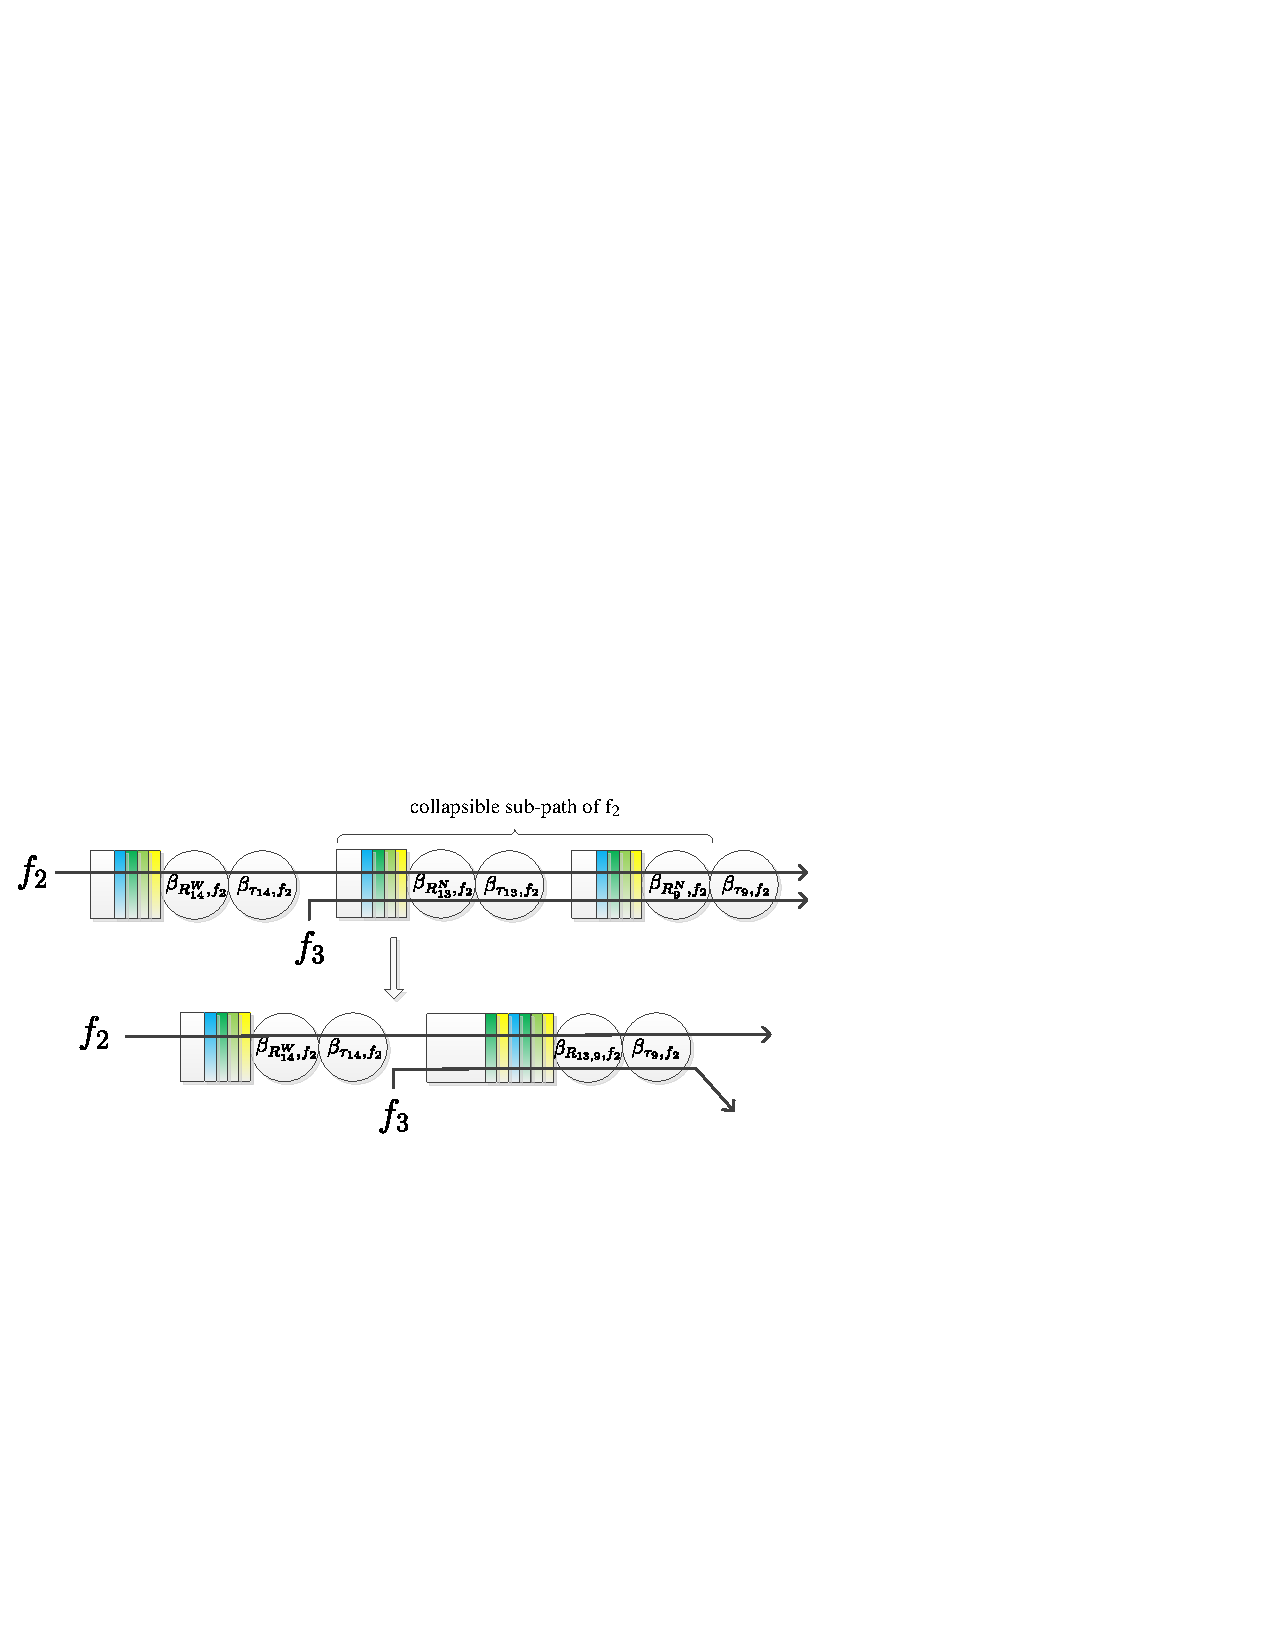
\includegraphics[scale=0.6]{fig8.pdf}\\
  \caption{Collapsible sub-path of $f_2$. Since the flow control between $R_{13}$ and $R_9$ can be neglected, they are replaced by a single virtual router $R_{13,9}$.}\label{collapse}
\end{figure}

We formalize this observation and propose the concept of Collapsible Sub-Path (CSP) to simplify the calculation and improve the tightness of the delay bound.

\begin{rmk}[Collapsible Sub-Path]\label{csp}
Supposing the buffer size at each router is sufficient large so that there is no blocking caused by flow control in the network. Then, a CSP of flow $f_i$ (denoted as $\mathcal{C}_i$) is a sub-sequence of $\mathcal{R}_i$ satisfying the following conditions:
\begin{enumerate}
  \item for any router $R_j\in \mathcal{C}_i$, $|\Omega_{R_j,f_i}|\geq 1$.
  \item for any two distinct routers $R_j,R_k\in \mathcal{C}_i$, $\Theta_{R_j,f_i}=\Theta_{R_k,f_i}$ and $\Omega_{R_j,f_i}=\Omega_{R_k,f_i}$.
\end{enumerate}
\end{rmk}

The first condition indicates that we should compute the leftover service curve on this sub-path since there exists lower priority flows than $f_i$. The second condition ensures that the routers on this sub-path are shared by all the contending flows and the sub-path contains at least two routers.

According to definition \ref{csp}, we know that each flow may have several CSPs. Denote the set of all the CSPs of flow $f_i$ as $\mathcal{CSP}(f_i)$, we can first construct $\mathcal{CSP}(f_i)$ by scanning $\mathcal{R}_i$. Then, for each $\mathcal{C}_j\in\mathcal{CSP}(f_i)$, we replace all the routers in $\mathcal{C}_j$ with a single virtual router providing RTC service curve $<\otimes_{R_k\in \mathcal{C}_j}\beta_{R_k,f_i}^l,\otimes_{R_k\in \mathcal{C}_j}\beta_{R_k,f_i}^u>$. For a CSP with $n$ ($n\geq 2$) routers, this method reduces $n-1$ times calculation of intermediate RTC arrival curve and leftover service curve when compared to the router-by-router calculation as Alg. \ref{alg:equivalentservicecurve}. In addition, the tightness of delay bound is also improved due to the well-known ``pay burst only once" property of DNC theory.

This idea is summarized as Alg. \ref{improvedalg}. An example is presented in Fig. \ref{example} to illustrate the basic step of this algorithm.
\begin{algorithm}
\caption{Improved end-to-end delay analysis algorithm}\label{improvedalg}
\begin{algorithmic}[1]
\Require Architecture parameters and flow specifications
\Ensure Worst-case end-to-end delay for all the flows
    \For {each flow $f_i\in \mathcal{F}$ with priority order}
        \State // Compute the service curve at each router for $f_i$
        \For {each router $R_j\in \mathcal{R}_{i}$ from $end_i$ to $start_i$}
            \State $\beta_{R_j^\prime,f_i}^l=\beta_{BW}^l\otimes\beta_{RC}^l\otimes\beta_{VA}^l\otimes\beta_{SA}^l\otimes\lfloor\frac{\beta_{ST,R_j^{p}}^{l^\prime}}{|\Theta_{R_j,f_i}|+1}\rfloor$;
            \State $\beta_{R_j^\prime,f_i}^u=\beta_{BW}^u\otimes\beta_{RC}^u\otimes\beta_{VA}^u\otimes\beta_{SA}^u\otimes\lceil\frac{\beta_{ST,R_j^{p}}^{u^\prime}}{|\Theta_{R_j,f_i}|+1}\rceil$;
        \EndFor
        \State Construct $\mathcal{CSP}(f_i)$ and update $\mathcal{R}_i$
        \State // Compute the leftover service curve for low-priority flows
        \State $\beta_{f_i}^l=\beta_{NI,f_i}^l$; $\beta_{f_i}^u=\beta_{NI,f_i}^u$;
        \For {$\forall R_j\in\mathcal{R}_{i}$ from $start_i$ to $end_i$}
            \If {$\Omega_{R_j,f_i}\neq \emptyset$}
                \State $\beta^l=\beta^l_{f_i}\otimes\beta_{BW}^l\otimes\beta_{RC}^l\otimes\beta_{VA}^l\otimes\beta_{SA}^l$;
                \State $\beta^u=\beta^u_{f_i}\otimes\beta_{BW}^u\otimes\beta_{RC}^u\otimes\beta_{VA}^u\otimes\beta_{SA}^u$;
                \State //Compute the arrival curve of $f_i$ at $R_j$
                \State $\alpha^l_{R_j,f_i}=\min\{(\alpha^l_{f_i}\oslash\beta^u)\otimes\beta^l,\beta^l\}$;
                \State $\alpha^u_{R_j,f_i}=\min\{(\alpha^u_{f_i}\otimes\beta^u)\oslash\beta^l,\beta^u\}$;
                \If {$Delay(f_k)$ has been calculated for $\forall f_k\in\Theta_{R_j,f_i}$}
                    \State $\alpha^l_{R_j,f_i}=\alpha^l_{R_j,f_i}+\sum_{f_k\in\Theta_{R_j,f_i}}\alpha^l_{R_j,f_k}$;
                    \State $\alpha^u_{R_j,f_i}=\alpha^u_{R_j,f_i}+\sum_{f_k\in\Theta_{R_j,f_i}}\alpha^u_{R_j,f_k}$;
                    \State $\beta^{l^\prime}_{ST,R_j^{p}}=(\beta^{l^\prime}_{ST,R_j^{p}}-\alpha^u_{R_j,f_i})\bar{\otimes}0$;
                    \State $\beta^{u^\prime}_{ST,R_j^{p}}=\max\{(\beta^{u^\prime}_{ST,R_j^{p}}-\alpha^l_{R_j,f_i})\bar{\oslash}0,0\}$;
                \EndIf
            \EndIf
            \State $\beta_{f_i}^l=\beta_{f_i}^l\otimes\beta^l_{R_j^\prime,f_i}\otimes\beta^l_{LT}$; $\beta_{f_i}^u=\beta_{f_i}^u\otimes\beta^u_{R_j^\prime,f_i}\otimes\beta^u_{LT}$;
        \EndFor
        \State // Compute the end-to-end delay for $f_i$
        \State $Delay(f_i)=H(\alpha^u_{f_i},\beta_{NI,f_i}^l\otimes (\underset{R_k\in\mathcal{R}_{i}}{\bigotimes}(\beta^l_{R_k^\prime,f_i}\otimes\beta^l_{LT})))$;
    \EndFor
\end{algorithmic}
\end{algorithm}

\subsection{Buffer Sizing Algorithm}\label{bufferopt}
The priority-aware wormhole-switched NoC \cite{Shi:2008:RCA:1397757.1397996}\cite{189}\cite{73} requires the same amount of VCs as the priorities to prevent priority inversion, which refers to the blocking of high-priority flows when the low priority flows occupy all the VCs \cite{707545}. To reduce the buffer area and power consumption of priority-aware wormhole-switched NoC, VC sharing \cite{5161497} and buffer optimization \cite{189} techniques have been proposed. The VC sharing scheme \cite{5161497} reduces the total VC number by allowing an VC shared by multiple flows. However, this sharing will lead to performance degradation and even deadlock under some routing polices. Thus, we keep the VC number unchanged and try to reduce the VC depth, as done in \cite{189}. The backlog bound of each router derived in \cite{189} is the minimum buffer size that does not trigger the flow control. Reducing this buffer size further will cause the back-pressure between adjacent routers and lead to a larger end-to-end delay. But, it is feasible to do so as long as the deadline constraint of each flow is not violated. Thus, we propose a buffer sizing algorithm to further reduce the initial buffer size of each router until the end-to-end delay of a flow violates its deadline or the buffer size is equal to one. We set the initial buffer size to a small value which is sufficient to avoid flow control. This value can be obtained by applying the following theorem.
\begin{thm}\label{initial}
Denote by $\beta_{R_j,f_i}^l$ the basic feed-forward lower service curve obtained at $R_j\in\mathcal{R}_i$ by flow $f_i$, $\beta_{LT}^l$ the lower service curve provided by the physical link between two adjacent routers, $B_{R_j,f_i}$ the VC buffer size reserved for $f_i$ at $R_j$ and $\sigma$ the credit feedback delay. Then, for $\forall R_j\in\mathcal{R}_i$, the buffer size $$B_{R_j,f_i}=\lceil\inf\{B|\beta_{R_j,f_i}^l\otimes\beta_{LT}^l\otimes\overline{\beta_{R_j,f_i}^l\otimes\beta_{LT}^l\otimes\delta_\sigma(t)+B}\geq\beta_{R_j,f_i}^l\otimes\beta_{LT}^l\}\rceil$$
is large enough to avoid flow control.
\end{thm}
\begin{pf}
We take the flow $f_2$ in Fig. \ref{f2} as an example to verify this theorem. As stated by Theorem \ref{credit}, we have $$\beta_{FC,R_9,f_2}^l=\overline{\beta^l_{LT}\otimes\beta_{R_5,f_2}^l\otimes\delta_\sigma+B_{R_5,f_2}}$$ and
\begin{eqnarray*}
\beta_{FC,R_{13},f_2}^l&=&\overline{\beta^l_{LT}\otimes\beta^l_{R_9,f_2}\otimes\overline{\beta^l_{LT}\otimes\beta^l_{R_5,f_2}\otimes\delta_\sigma+B_{R_5,f_2}}\otimes\delta_\sigma+B_{R_9,f_2}}\label{eq1}\\
&=&\overline{(\beta^l_{LT}\otimes\beta^l_{R_9,f_2}\otimes\delta_\sigma+B_{R_9,f_2})\otimes\overline{\beta^l_{LT}\otimes\beta^l_{R_5,f_2}\otimes\delta_\sigma+B_{R_5,f_2}}}\label{eq2}\\
&=&\overline{\beta^l_{LT}\otimes\beta^l_{R_9,f_2}\otimes\delta_\sigma+B_{R_9,f_2}}\otimes\overline{\beta^l_{LT}\otimes\beta^l_{R_5,f_2}\otimes\delta_\sigma+B_{R_5,f_2}}\label{eq3}
\end{eqnarray*}
where these two steps hold due to the property P2 and P5 of $\otimes$ operator.

Similarly, we can prove that
$$\beta_{FC,R_{14},f_2}^l=\overline{\beta^l_{LT}\otimes\beta^l_{R_{13},f_2}\otimes\delta_\sigma+B_{R_{13},f_2}}\otimes\beta_{FC,R_{13},f_2}^l,$$
$$\beta_{FC,R_{15},f_2}^l=\overline{\beta^l_{LT}\otimes\beta^l_{R_{14},f_2}\otimes\delta_\sigma+B_{R_{13},f_2}}\otimes\beta_{FC,R_{14},f_2}^l,$$
$$\beta_{FC,NI,f_2}^l=\overline{\beta^l_{LT}\otimes\beta^l_{R_{15},f_2}\otimes\delta_\sigma+B_{R_{15},f_2}}\otimes\beta_{FC,R_{15},f_2}^l.$$

Then, the equivalent end-to-end feedback service curve obtained by $f_2$ is
\begin{eqnarray*}
\beta_{f_2}^l&=&\beta_{NI,f_2}^l\otimes\beta_{FC,NI,f_2}^l\otimes(\underset{R_j\in\mathcal{R}_2}{\bigotimes}(\beta^l_{R_j,f_2}\otimes\beta^l_{FC,R_j,f_2}\otimes\beta_{LT}^l))\\
&=& \beta_{NI,f_2}^l\otimes(\underset{R_j\in\mathcal{R}_2}{\bigotimes}(\beta^l_{R_j,f_2}\otimes\beta_{LT}^l))\otimes(\beta_{FC,NI,f_2}^l\otimes(\underset{R_j\in\mathcal{R}_2}{\bigotimes}\beta_{FC,R_j,f_2}))\\
&=& \beta_{NI,f_2}^l\otimes(\underset{R_j\in\mathcal{R}_2}{\bigotimes}(\beta^l_{R_j,f_2}\otimes\beta_{LT}^l))\otimes(\underset{R_j\in\mathcal{R}_2}{\bigotimes}\overline{\beta_{R_j,f_2}\otimes\beta_{LT}\otimes\delta_\sigma+B_{R_j,f_2}})\\
&=& \beta_{NI,f_2}^l\otimes(\underset{R_j\in\mathcal{R}_2}{\bigotimes}(\beta^l_{R_j,f_2}\otimes\beta_{LT}^l\otimes\overline{\beta^l_{LT}\otimes\beta^l_{R_{j},f_2}\otimes\delta_\sigma+B_{R_j,f_2}}))
\end{eqnarray*}
where the second line and the fourth line hold due to the commutativity of min-plus convolution.

We know that when the buffer size is large enough, the effectiveness of flow controller to the RTC service curve is eliminated and the equivalent RTC service curve obtained at subsection 4.3 is equal to the basic feed-forward service curve derived in subsection 4.2.2. According to the property P8 of $\otimes$ operator, we know that
\begin{equation}\label{sufficient}
\beta_{R_j,f_2}^l\otimes\beta_{LT}^l\otimes\overline{\beta_{R_j,f_2}^l\otimes\beta_{LT}^l\otimes\delta_\sigma(t)+B_{R_j,f_2}}\geq\beta_{R_j,f_2}^l\otimes\beta_{LT}^l,\forall R_j\in\mathcal{R}_2
\end{equation}
is a sufficient condition for
$$\beta_{f_2}^l\geq\beta_{NI,f_2}^l\otimes(\underset{R_j\in\mathcal{R}_2}{\bigotimes}(\beta^l_{R_j,f_2}\otimes\beta_{LT}^l))$$ where the right side of the above inequality is the basic end-to-end feed-forward service curve provided to $f_2$. Thus, to avoid flow control, the buffer size at each router reserved for flow $f_2$ can be assigned to the minimum integer value to make Eq.(\ref{sufficient}) hold, which ends the proof. \hspace*{\fill}~\QED\par\endtrivlist\unskip
\end{pf}

Suppose that the applications have been mapped onto the NoC, and each flow $f_i$ has been assigned to their corresponding priority $P_i$ and deadline $D_i$. Following the same notation as Algorithm \ref{alg:equivalentservicecurve}, we propose the buffer sizing algorithm to allocate just enough buffer for each flow along its routine to meet their deadline constraint, as shown in Algorithm \ref{alg:bufopt}. We assume that the service curve provided by the source NI of $f_i$,i.e. $<\beta_{NI,f_i}^l,\beta_{NI,f_i}^u>$, has been computed with Algorithm \ref{alg:scatni}.
\begin{algorithm}[!ht]
\caption{Buffer sizing algorithm}
\label{alg:bufopt}
\begin{algorithmic}[1]
\Require Architecture parameters and flow specifications
\Ensure Buffer required for each flow to meet their deadline
    \For {each flow $f_i\in \mathcal{F}$ with priority order}
        \For {each router $R_j\in \mathcal{R}_{i}$ from $end_i$ to $start_i$}
            \State $\beta_{FC,R_j,f_i}^l=\delta_0(t)$; $\beta_{FC,R_j,f_i}^u=\delta_0(t)$;
            \State $\beta_{R_j^\prime,f_i}^l=\beta_{BW}^l\otimes\beta_{RC}^l\otimes\beta_{VA}^l\otimes\beta_{SA}^l\otimes\lfloor\frac{\beta_{ST,R_j^{p}}^{l^\prime}}{|\Theta_{R_j,f_i}|+1}\rfloor\otimes\beta_{FC,R_j,f_i}^l$;
            \State $\beta_{R_j^\prime,f_i}^u=\beta_{BW}^u\otimes\beta_{RC}^u\otimes\beta_{VA}^u\otimes\beta_{SA}^u\otimes\lceil\frac{\beta_{ST,R_j^{p}}^{u^\prime}}{|\Theta_{R_j,f_i}|+1}\rceil\otimes\beta_{FC,R_j,f_i}^u$;
            \State compute the initial buffer size $B_{R_j,f_i}$ according to Theorem \ref{initial};
        \EndFor
        \State $\beta_{FC,NI,f_i}^l=\delta_0(t)$; $\beta_{FC,NI,f_i}^u=\delta_0(t)$;
        \State Buffer\_Reduction($\alpha^u_{f_i},\mathcal{R}_i,D_i$);\Comment Call the Buffer\_Reduction procedure
        \State $\beta_{f_i}^l=\beta_{NI,f_i}^l\otimes\beta_{FC,NI,f_i}^l$; $\beta_{f_i}^u=\beta_{NI,f_i}^u\otimes\beta_{FC,NI,f_i}^u$;
        \For {$\forall R_j\in\mathcal{R}_{i}$ from $start_i$ to $end_i$}
            \If {$\Omega_{R_j,f_i}\neq \emptyset$}
                \State $\beta^l=\beta^l_{f_i}\otimes\beta_{BW}^l\otimes\beta_{RC}^l\otimes\beta_{VA}^l\otimes\beta_{SA}^l$;
                \State $\beta^u=\beta^u_{f_i}\otimes\beta_{BW}^u\otimes\beta_{RC}^u\otimes\beta_{VA}^u\otimes\beta_{SA}^u$;
                \State $\alpha^l_{R_j,f_i}=\min\{(\alpha^l_{f_i}\oslash\beta^u)\otimes\beta^l,\beta^l\}$;
                \State $\alpha^u_{R_j,f_i}=\min\{(\alpha^u_{f_i}\otimes\beta^u)\oslash\beta^l,\beta^u\}$;
                \If {$\forall f_k\in\Theta_{R_j,f_i}$, $Delay(f_k)$ has been calculated}
                    \State $\alpha^l_{R_j,f_i}=\alpha^l_{R_j,f_i}+\sum_{f_k\in\Theta_{R_j,f_i}}\alpha^l_{R_j,f_k}$;
                    \State $\alpha^u_{R_j,f_i}=\alpha^u_{R_j,f_i}+\sum_{f_k\in\Theta_{R_j,f_i}}\alpha^u_{R_j,f_k}$;
                    \State $\beta^{l^\prime}_{ST,R_j^{p}}=(\beta^{l^\prime}_{ST,R_j^{p}}-\alpha^u_{R_j,f_i})\bar{\otimes}0$;
                    \State $\beta^{u^\prime}_{ST,R_j^{p}}=\max\{(\beta^{u^\prime}_{ST,R_j^{p}}-\alpha^l_{R_j,f_i})\bar{\oslash}0,0\}$;
                \EndIf
            \EndIf
            \State $\beta_{f_i}^l=\beta_{f_i}^l\otimes\beta^l_{R_j^\prime,f_i}\otimes\beta^l_{LT}$; $\beta_{f_i}^u=\beta_{f_i}^u\otimes\beta^u_{R_j^\prime,f_i}\otimes\beta^u_{LT}$;
        \EndFor
    \EndFor
\end{algorithmic}
\end{algorithm}

Our algorithm tries to reduce the buffer size for each flow from high-priority to low-priority iteratively. For each iteration, it performs the following four steps: (1) Calculate the basic feed-forward service curves provided by the routers (lines 3-5). (2) Calculate the initial buffer size to avoid flow control for each router (line 6). (3) Reduce the initial buffer size gradually as long as the constraint of deadline is not being violated (line 9). This step is abstracted as a procedure, i.e. Buffer\_Reduction($f_i$). This procedure tries to reduce the buffer size of each router reserved for the target flow $f_i$ from its ejection router to its injection router. For each router on the path of $f_i$, it decreases the buffer size iteratively, until the buffer size is reduced to one or the deadline constraint is violated. If the iteration stops due to the violation of deadline, the buffer size and related service curves are restored to their previous value. To ease the description, we define the operator $Pre(R_j)$ to identify the predecessor of router $R_j$, and let $Pre(start_i)=NI$. (4) Calculate the leftover service curve at each router for low-priority flows (lines 10-25). The computation complexity of the Buffer\_Reduction($f_i$) procedure and the entire buffer sizing algorithm are $O(H^2)$ and $O(NH^2)$, where $N$ and $H$ denote the number of flows analyzed and the maximum hop count of these flows. This algorithm can be implemented in RTC toolbox \cite{rtc} to optimize the buffer size automatically.
\begin{algorithm}
\begin{algorithmic}[1]
%\Require Architecture parameters and flow specifications
%\Ensure $B_{R_j,f_i}$ //buffer size reserved at each router for $f_i$
\Procedure{Buffer\_Reduction}{$\alpha^u_{f_i},\mathcal{R}_i,D_i$}
        \For {each router $R_j\in \mathcal{R}_{i}$ from $end_i$ to $start_i$}
            \State $Delay(f_i)=H(\alpha_{f_i}^u,\beta_{NI,f_i}^l\otimes\beta^l_{FC,NI,f_i}\otimes (\underset{R_k\in\mathcal{R}_{i}}{\bigotimes}(\beta^l_{R_k^\prime,f_i}\otimes\beta^l_{LT})))$;
            \While {$Delay(f_i)\leq D_i$ and $B_{R_j,f_i}>1$}
                \State $B_{R_j,f_i}=B_{R_j,f_i}-1$;
                \For {all $R_{k}\in\mathcal{R}_i$ from $Pre(R_j)$ to $start_i$}
                    \State compute $<\beta_{FC,R_k,f_i}^l,\beta_{FC,R_k,f_i}^u>$ according to Theorem \ref{credit};
                    \State compute the service curve $<\beta_{R_k^\prime,f_i}^l,\beta_{R_k^\prime,f_i}^u>$;
                \EndFor
                \State compute the service curve $<\beta_{FC,NI,f_i}^l,\beta_{FC,NI,f_i}^u>$;
                \State $Delay(f_i)=H(\alpha_{f_i}^u,\beta_{NI,f_i}^l\otimes\beta^l_{FC,NI,f_i}\otimes (\underset{R_k\in\mathcal{R}_{i}}{\bigotimes}(\beta^l_{R_k^\prime,f_i}\otimes\beta^l_{LT})))$;
            \EndWhile
            \If {$Delay(f_i)>D_i$}
                \State $B_{R_j,f_i}=B_{R_j,f_i}+1$;
                \State recompute $<\beta_{FC,Pre(R_j),f_i}^l,\beta_{FC,Pre(R_j),f_i}^u>$;
                \State recompute $<\beta_{Pre(R_j),f_i}^l,\beta_{Pre(R_j),f_i}^u>$ if $R_j\neq start_i$;
            \EndIf
        \EndFor
\EndProcedure
\end{algorithmic}
\end{algorithm}

The number of cycles that a packet can be delayed in the network without violating its deadline is referred to `slack' in \cite{6560630}. Thus, the Buffer\_Reduction procedure of our buffer sizing algorithm is the process of slack minimization. However, while used for power reduction, our buffer sizing algorithm is significantly different from the DNC-based slack optimization algorithm proposed in \cite{6560630}. In \cite{6560630}, the energy optimization is achieved by adjusting the voltage, frequency and link bandwidth of on-chip routers for the fixed configuration and deadline. In contrast, our method tries to reduce the buffer size under the deadline constraint, and the buffer reduction directly leads to the area and power saving. In addition, our algorithm can be also used in conjunction with the priority sharing techniques \cite{5161497} to minimize the hardware cost of priority-aware wormhole-switched NoC.


\section{Experiments}\label{experiments}
In this section, we validate the correctness and tightness of our performance model by comparing with simulation results and other analytical methods. There is extensive research on the buffer sizing problem of the priority-aware NoC, representative methods include shaping delay analysis \cite{Manolache:2006:BSO:1131481.1131683}, FLBA and LLBA \cite{189}. We will only perform the comparison with LLBA in subsection 5.1 since it gives lower buffer space bound than FLBA and shaping delay analysis. There are also several analytical methods exist for the delay analysis of priority-aware NoC, examples include lumped link model \cite{707545}, dependency graph model \cite{708526}, contention tree model \cite{LuJS05}, Rate Monotonic (RM) method \cite{365629}, FLA \cite{Shi:2008:RCA:1397757.1397996}, LLA \cite{73} and DNC \cite{Qian489900}, etc. Among all these methods, LLA and DNC outperform the others when the tightness of delay bound is considered. Thus, we will only compare our delay analysis algorithms with LLA and DNC, as presented in subsection 5.2. We also present the simulation results to validate the correctness and tightness of our method in subsection \ref{sim}.

Throughout this section, we compare our analytical results with those obtained by other analytical methods and simulation under a $4\times 4$ mesh network. The applications we choose include the synthesis traffic pattern shown in Fig. \ref{topology} and two real-world applications, i.e. autonomous vehicle \cite{Shi2009} and errison radio \cite{Jafari1922089,LuJa08} applications. The autonomous vehicle applications consists of 38 flows mapped onto a $4\times 4$ mesh network. The flow ID ($f_i$), priority ($P_i$), source address (Src), destination address (Dst), packet length ($F_i$, in flits) and injection period ($I_i$, in $10^6$ cycles) of each flow in this application are presented in Table \ref{vehicle}. The errison application is comprised of 16 IP cores and 26 communication flows. These flows are classified into nine groups with each group has different bandwidth requirement, as shown in Fig. \ref{trafficpattern}.
\begin{table}[htbp]
\centering
\caption{\label{vehicle}Flow specification of autonomous vehicle benchmark}
\begin{tabular}{|c|c|c|c|c|c||c|c|c|c|c|c|c|c|}
\hline
$f_i$ & $P_i$ & Src &��Dst & $F_i$ & $I_i$ & $f_i$ & $P_i$ & Src &��Dst & $F_i$ & $I_i$\\
\hline
1 & 31 & 1 & 6 & 1024 & 50 & 2 & 32 & 6 & 9 & 2048 & 50\\
\hline
3 & 33 & 9 & 6 & 16384 & 50 & 4 & 34 &9 & 5 & 16384 & 50\\
\hline
5 & 24 & 6 & 16 & 512 & 10 & 6 & 25 & 12 & 6 & 512 & 10\\
\hline
7 & 26 & 6 & 14 & 1024 & 10 & 8 & 1 & 9 & 2 & 38400 & 4\\
\hline
9 & 2 & 16 & 15 & 38400 & 4 & 10 & 3 & 2 & 6 & 512 & 4\\
\hline
11 & 4 & 15 & 6 & 512 & 4 & 12 & 5 & 1 & 2 & 38400 & 4\\
\hline
13 & 6 & 5 & 6 & 38400 & 4 & 14 & 7 & 9 & 10 & 38400 & 4\\
\hline
15 & 8 & 13 & 14 & 38400 & 4 & 16 & 9 & 4 & 7 & 38400 & 4\\
\hline
17 & 10 & 8 & 7 & 38400 & 4 & 18 & 11 & 12 & 11 & 38400 & 4\\
\hline
19 & 12 & 16 & 15 & 38400 & 4 & 20 & 13 & 2 & 7 & 2048 & 4\\
\hline
21 & 14 & 6 & 7 & 2048 & 4 & 22 & 15 & 10 & 7 & 2048 & 4\\
\hline
23 & 16 & 14 & 7 & 2048 & 4 & 24 & 17 & 3 & 10 & 2048 & 4\\
\hline
25 & 18 & 7 & 10 & 2048 & 4 & 26 & 19 & 11 & 12 & 2048 & 4\\
\hline
27 & 20 & 15 & 10 & 2048 & 4 & 28 & 21 & 7 & 11 & 8192 & 4\\
\hline
29 & 22 & 10 & 11 & 8192 & 4 & 30 & 23 & 11 & 5 & 4096 & 4\\
\hline
31 & 35 & 1 & 5 & 1024 & 50 & 32 & 27 & 13 & 5 & 1024 & 10\\
\hline
33 & 37 & 5 & 9 & 4096 & 100 & 34 & 36 & 13 & 8 & 2048 & 50\\
\hline
35 & 28 & 3 & 8 & 512 & 10 & 36 & 38 & 8 & 4 & 2048 & 100\\
\hline
37 & 29 & 12 & 8 & 1024 & 10 & 38 & 30 & 8 & 14 & 1024 & 10\\
\hline
\end{tabular}
\end{table}

\begin{table}
\begin{tabular}{|c|c|c|}
\hline
Group & Priority & Period (cycles)\\
\hline
a   &   1   &   16\\
\hline
b   &   2   &   125\\
\hline
c   &   3   &   125\\
\hline
d   &   4   &   32\\
\hline
e   &   5   &   125\\
\hline
f   &   6   &   500\\
\hline
g   &   7   &   256\\
\hline
h   &   8   &   16\\
\hline
i   &   9   &   125\\
\hline
\end{tabular}
\end{table}

\begin{figure}
  \centering
  % Requires \usepackage{graphicx}
  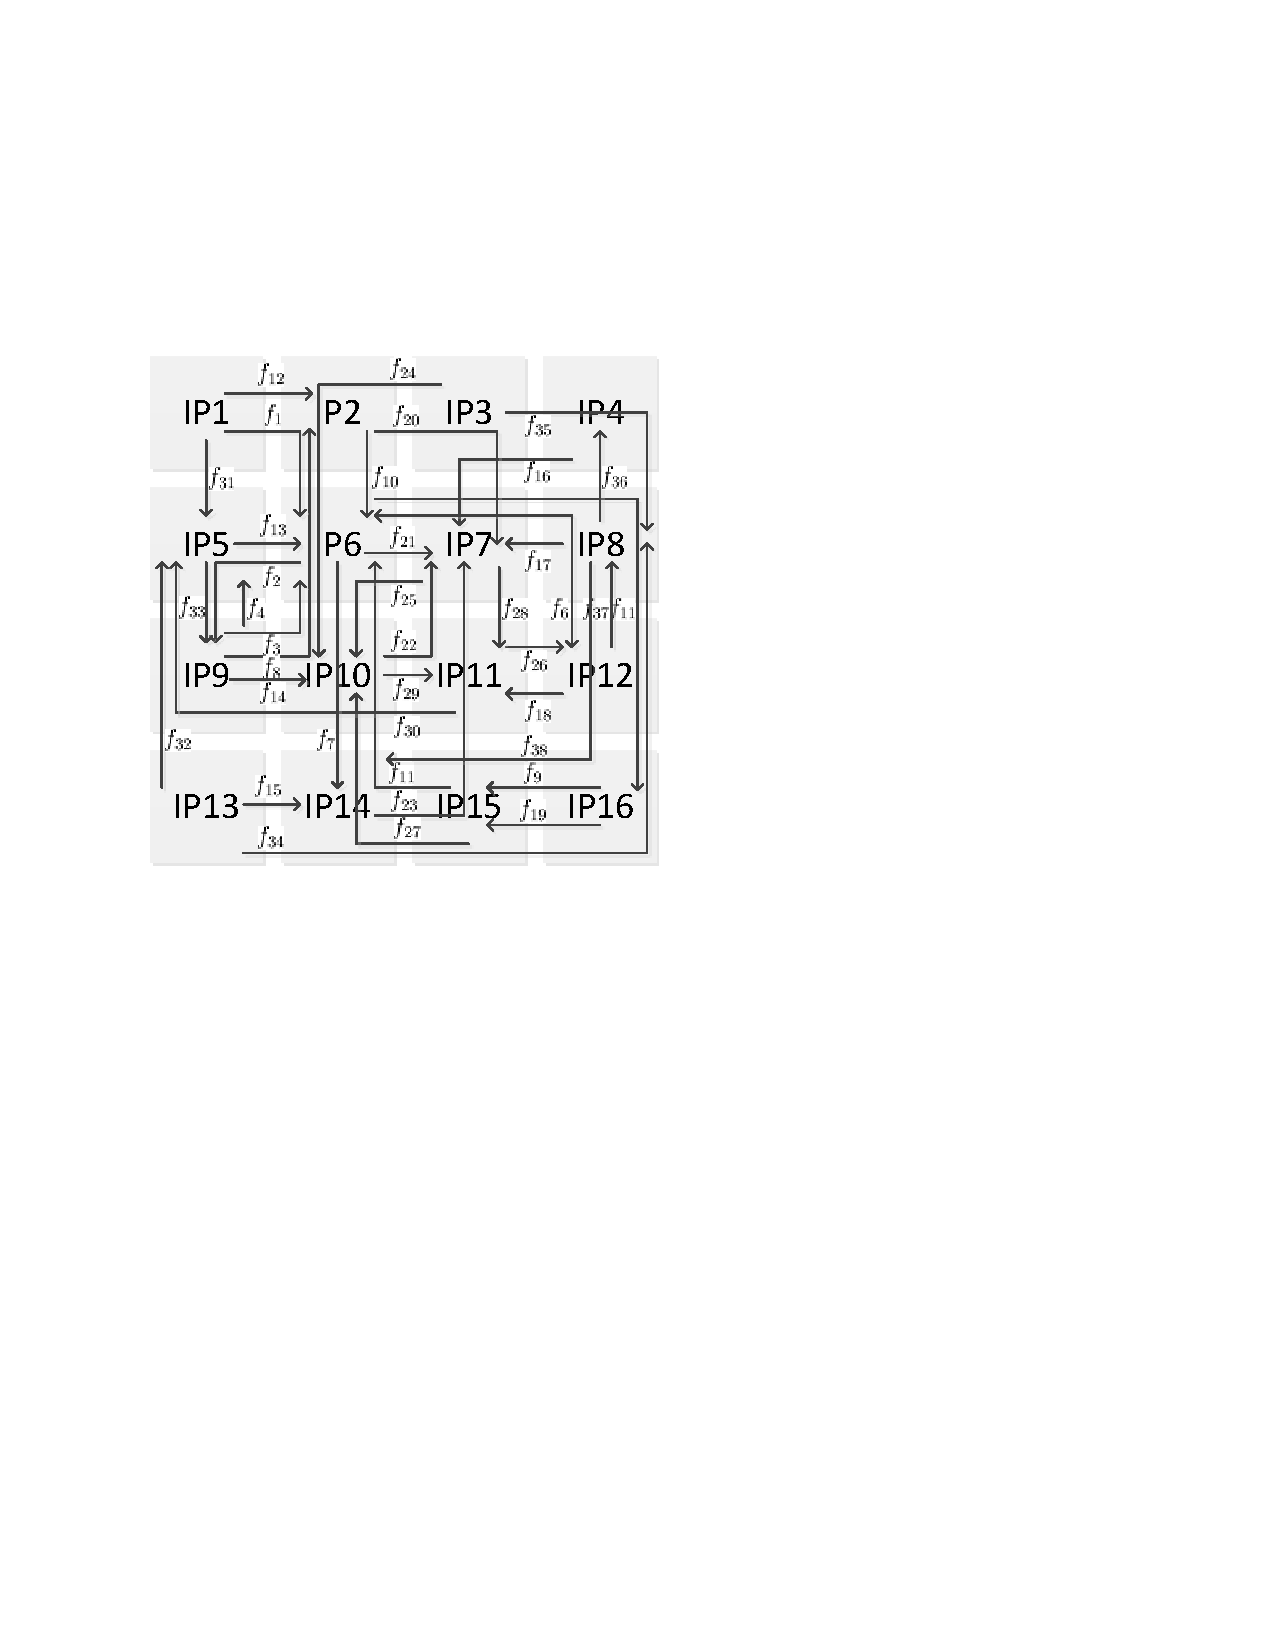
\includegraphics[scale=0.7]{fig9.pdf}\\
  \caption{Traffic pattern of ericsson radio system application}\label{trafficpattern}
\end{figure}

\subsection{Buffer Space Comparison}\label{llacmp}
There are four flows (i.e. $f_1$, $f_2$, $f_3$ and $f_4$) in the network shown in Fig. \ref{topology}, with different priorities $P_4>P_1>P_2>P_3$ ($f_4$ has the highest priority). We perform the comparison on a set of periodical traffic due to the restriction of LLBA method \cite{189}. The packet length (in flits) and injection period (in cycles) of flow $f_i$ ($i=1,2,3,4$) are denoted as $F_i$ and $I_i$, respectively. To ease the analysis of buffer requirement, the LLBA method assumes the number of bits in a flit is the same as the physical channel width, and the latency of a router is one cycle \cite{189}. Thus, our performance model for the standard wormhole-switched router should be specialized, which is achieved by letting the service curve of BW, RC, VA, SA and LT stage be a pair of burst delay function $<\delta_0(t),\delta_0(t)>$. Under this condition, the service curve of the entire router is equal to the service curve provided by the ST stage, which is $<\beta_{ST,R_i^p}^l,\beta_{ST,R_i^p}^u>$. The traffic jitter for all the flows are assumed to be zero for brevity and clarity. In addition, we set the credit feedback delay $\sigma=0$ cycle in our model since the LLBA method does not consider the influence of credit feedback delay on the buffer requirement.

Let us suppose that all the flows have the same packet injection period $I_i=50$ cycles and packet length $F_i=8$ flits ($i=1,2,3,4$). The delay bounds computed with the LLA method \cite{73} for these four flows are 21, 22, 21 and 13 cycles, respectively. We can also obtain the total buffer size reserved for the four flows (i.e. $f_1$, $f_2$, $f_3$ and $f_4$) with LLBA method \cite{189}, which are 11, 12, 18 and 4 flits, respectively. The total buffer size required by these four flows can be obtained by summing up the buffer size reserved for each flow along its path, which is 45 flits. This value is the minimum buffer space required for all these four flows to avoid the back-pressure caused by flow control. By allowing the flow control to be triggered, our buffer sizing algorithm can be utilized to reduce this buffer size further as long as the deadline constraint is not violated. Figure \ref{LLBAvsRTC} demonstrates the normalized buffer requirement calculated with LLBA and our method under different deadline constraint. It can be found that our method can give much tighter buffer estimation than LLBA, and the improvement of our method over LLBA becomes more and more significant as the deadline constraint is relaxed.
\begin{figure}
  \centering
  % Requires \usepackage{graphicx}
  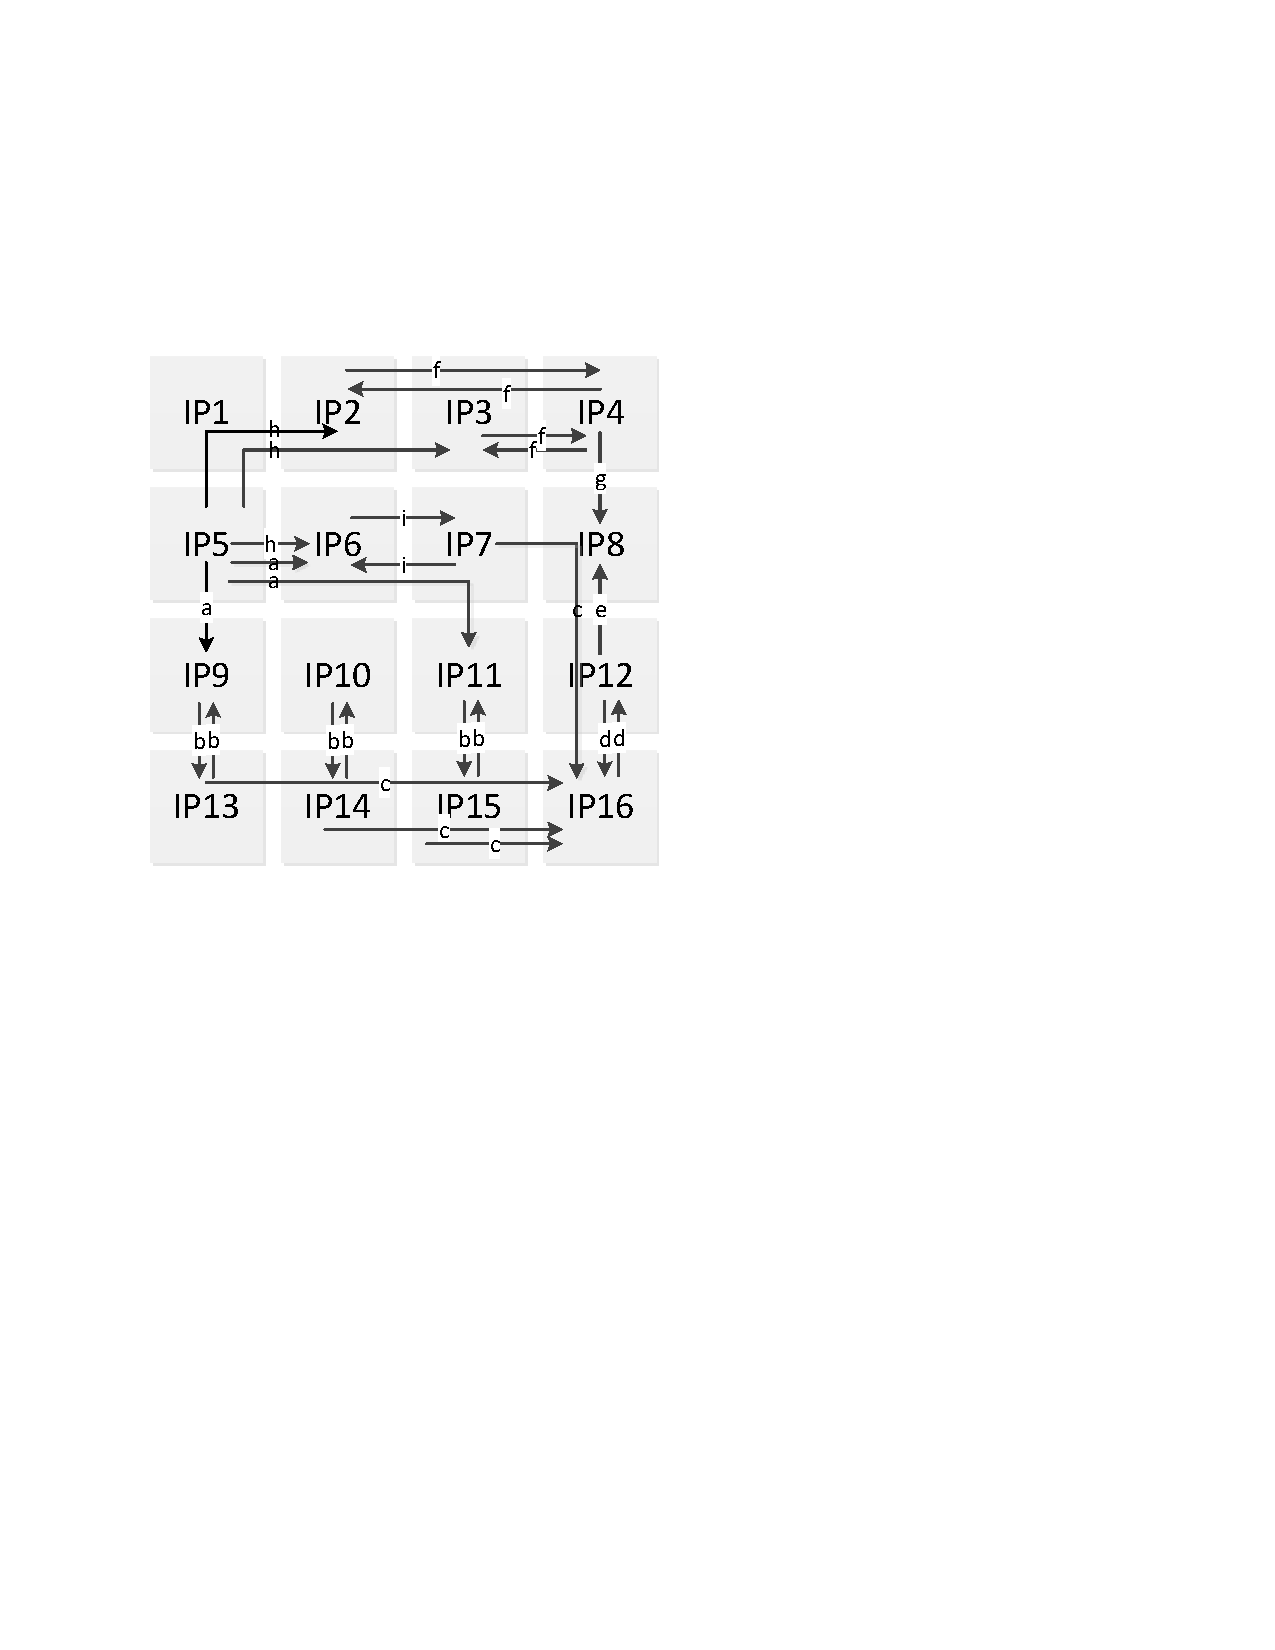
\includegraphics[scale=0.55]{fig10.pdf}\\
  \caption{Buffer requirement computed with our method for different deadline}\label{LLBAvsRTC}
\end{figure}


\subsection{Delay Bound Comparison}\label{dnccmp}

In this subsection, we present the numerical results to demonstrate the improvement of our method over the DNC method proposed in \cite{Qian489900}. The traffic pattern discussed in this subsection is shown in Fig. \ref{topology}. The priorities of these four flows (i.e. $f_1$, $f_2$, $f_3$ and $f_4$) in the network satisfy $P_4>P_1>P_2>P_3$. We perform the comparison on a set of periodical traffic. The packet length (in flits) and injection period (in cycles) of flow $f_i$ ($i=1,2,3,4$) are denoted as $F_i$ and $I_i$, respectively. The router architecture we considered in this subsection adopts the lookahead pipeline \cite{jerger2009chip}, which removes the RC stage from the critical path of the router pipeline. Thus, our service model is customized by letting the service curve of RC stage to be $<\delta_0(t),\delta_0(t)>$. The RTC arrival curve $<\alpha_{f_i}^l,\alpha_{f_i}^u>$ of flow $f_i$ can be obtained according to the method introduced in subsection \ref{traffic}. The DNC arrival curve for $f_i$ is $\alpha_{f_i}=V_i t+F_i$, where $V_i=F_i/I_i$ represents the average arrival rate.

We assume the VC buffer size of each router is $32$ flits, and the credit feedback delay $\sigma=0$ cycle. We change the injection rate $V_i$ ($i=1,2,3,4$) from $1/3$ to $1/6$ (flits/cycle) and the packet length $F_i$ from $1$ to $8$ flits. The end-to-end delay of flow $f_3$ calculated with the DNC method and our method are presented in Fig. \ref{comparison}. By comparison, we find that our method can give a much tighter delay bound than the DNC-based method proposed in \cite{Qian489900}. The root cause for this improvement lies in the fact that our method utilizes the upper service curve to limit the output upper arrival curve, which further leads to a tighter leftover service curve for the low-priority flows.
\begin{figure}
  \centering
  % Requires \usepackage{graphicx}
  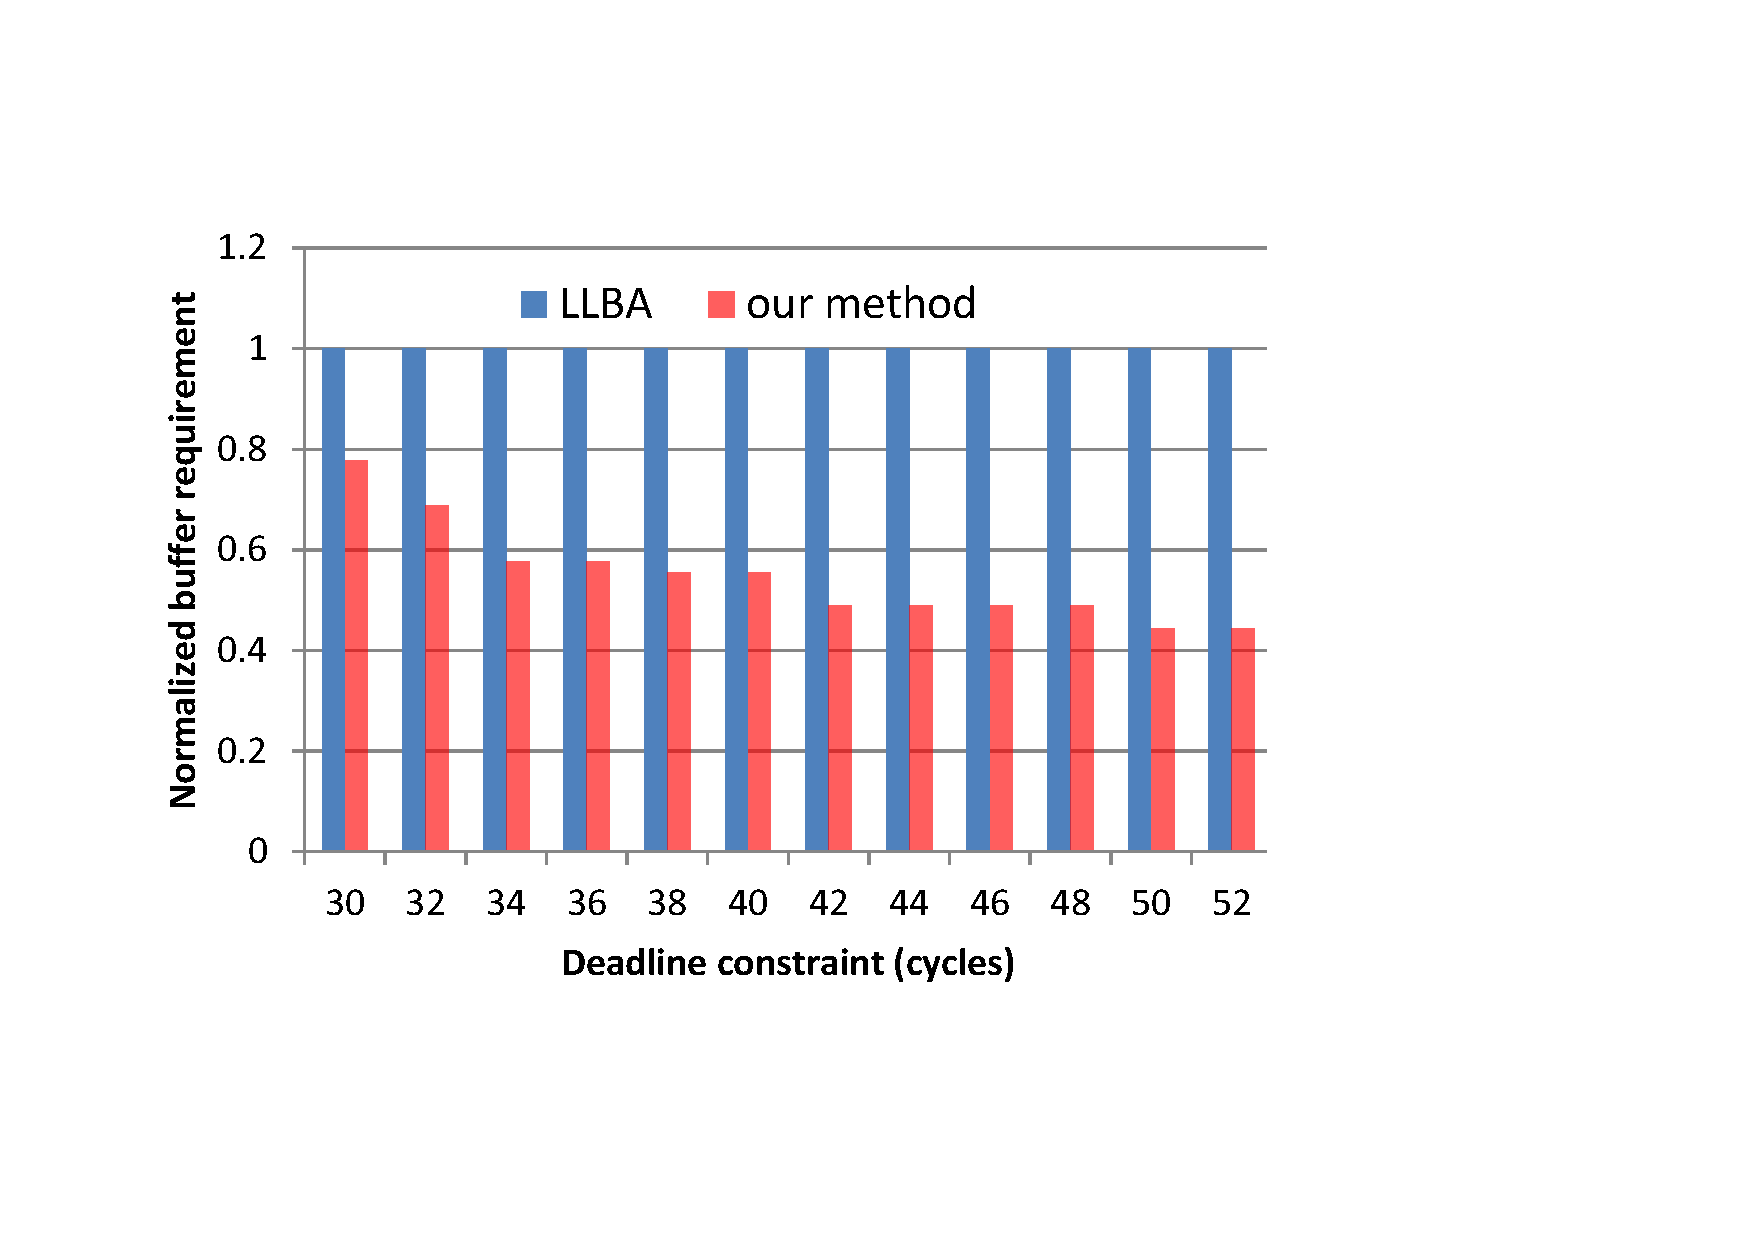
\includegraphics[scale=0.8]{fig11.pdf}\\
  \caption{Delay bound comparison with network calculus under different injection rate and packet length}\label{comparison}
\end{figure}

\subsection{Comparison with Simulation}\label{sim}

Our performance model is also verified by simulation. We modified the Booksim 2.0 \cite{6557149}, a cycle-accurate NoC simulator, to support the specified traffic pattern and injection process. The traffic patterns investigated in this subsection include the example shown in Fig. \ref{topology} and an real application provided by Ericsson Radio Systems \cite{LuJa08}\cite{Jafari1922089}. We adopt the optimized lookahead router \cite{jerger2009chip} to construct the mesh network. To fit this optimization, our service model is customized by letting the service curve of RC stage be $<\delta_0(t),\delta_0(t)>$. Other architecture and simulation parameters used in the simulation are listed in the Table \ref{arcpara}.
\begin{table}[htbp]
\centering
\caption{\label{arcpara}Architecture parameters used in the simulation}
\begin{tabular}{|c|c||c|c|}
\hline
network topology    & $4\times 4$ mesh  &   routing algorithm & X-Y routing\\
\hline
credit delay &  0 cycle &   channel width   & 128 bits\\
\hline
buffer size &   32 flits  &   switch allocator    &   priority-based\\
\hline
link latency    &   1 cycle    & sampling period &   $1\times 10^5$ cycles\\
\hline
clock cycle &   1 ns    &   warmup period   &   $3\times 10^5$ cycles\\
\hline
\end{tabular}
\end{table}

We first investigate the traffic pattern shown in Fig. \ref{topology}. Suppose that the injection process of each flow is the strictly periodical traffic without any jitter, and the priorities of these four flows satisfy $P_4>P_1>P_2>P_3$. However, even under this assumption, determining the worst-case delay by simulation for general scenarios is still a non-trivial task, because the worst-case delay of each flow depends on the traffic pattern and offset (i.e. the injection time of the first packet in a flow $f_i$, denoted as $O_i$) of all the flows in the network.

We set the injection rate $V_i$ ($i=1,2,3,4$) to $1/6$ (flits/cycle), and change the packet length $F_i$ from 2 flits to 9 flits. Under these conditions, we find that $f_1$ will experience the maximum delay in the network if its offset $O_1$ is equal to that of $f_4$. Similarly, the worst-case interference of $f_2$ occurs when its offset $O_2=O_1+(4+1)$, where $O_1+(4+1)$ is the time instance that the first packet of $f_1$ leaves router $R_{16}$, since the basic latency of a lookahead router and physical channel are 4 cycles and 1 cycles, respectively. Flow $f_3$ experiences the worst-case delay when $O_3=O_2+F_1+2\times(4+1)$. Thus, we set $O_1=O_4=0$ cycle, $O_2=5$ cycles, $O_3=15+F_1$ cycles, and run the simulation. The collected maximum end-to-end delay of these four flows under the given offset combination are compared with our RTC method, as shown in Fig. \ref{rtcvssim}. As indicated in this figure, for the given configurations, the delay bounds calculated with our method are indeed the upper bounds of simulation results, which verifies the correctness of our method.
\begin{figure}
  \centering
  % Requires \usepackage{graphicx}
  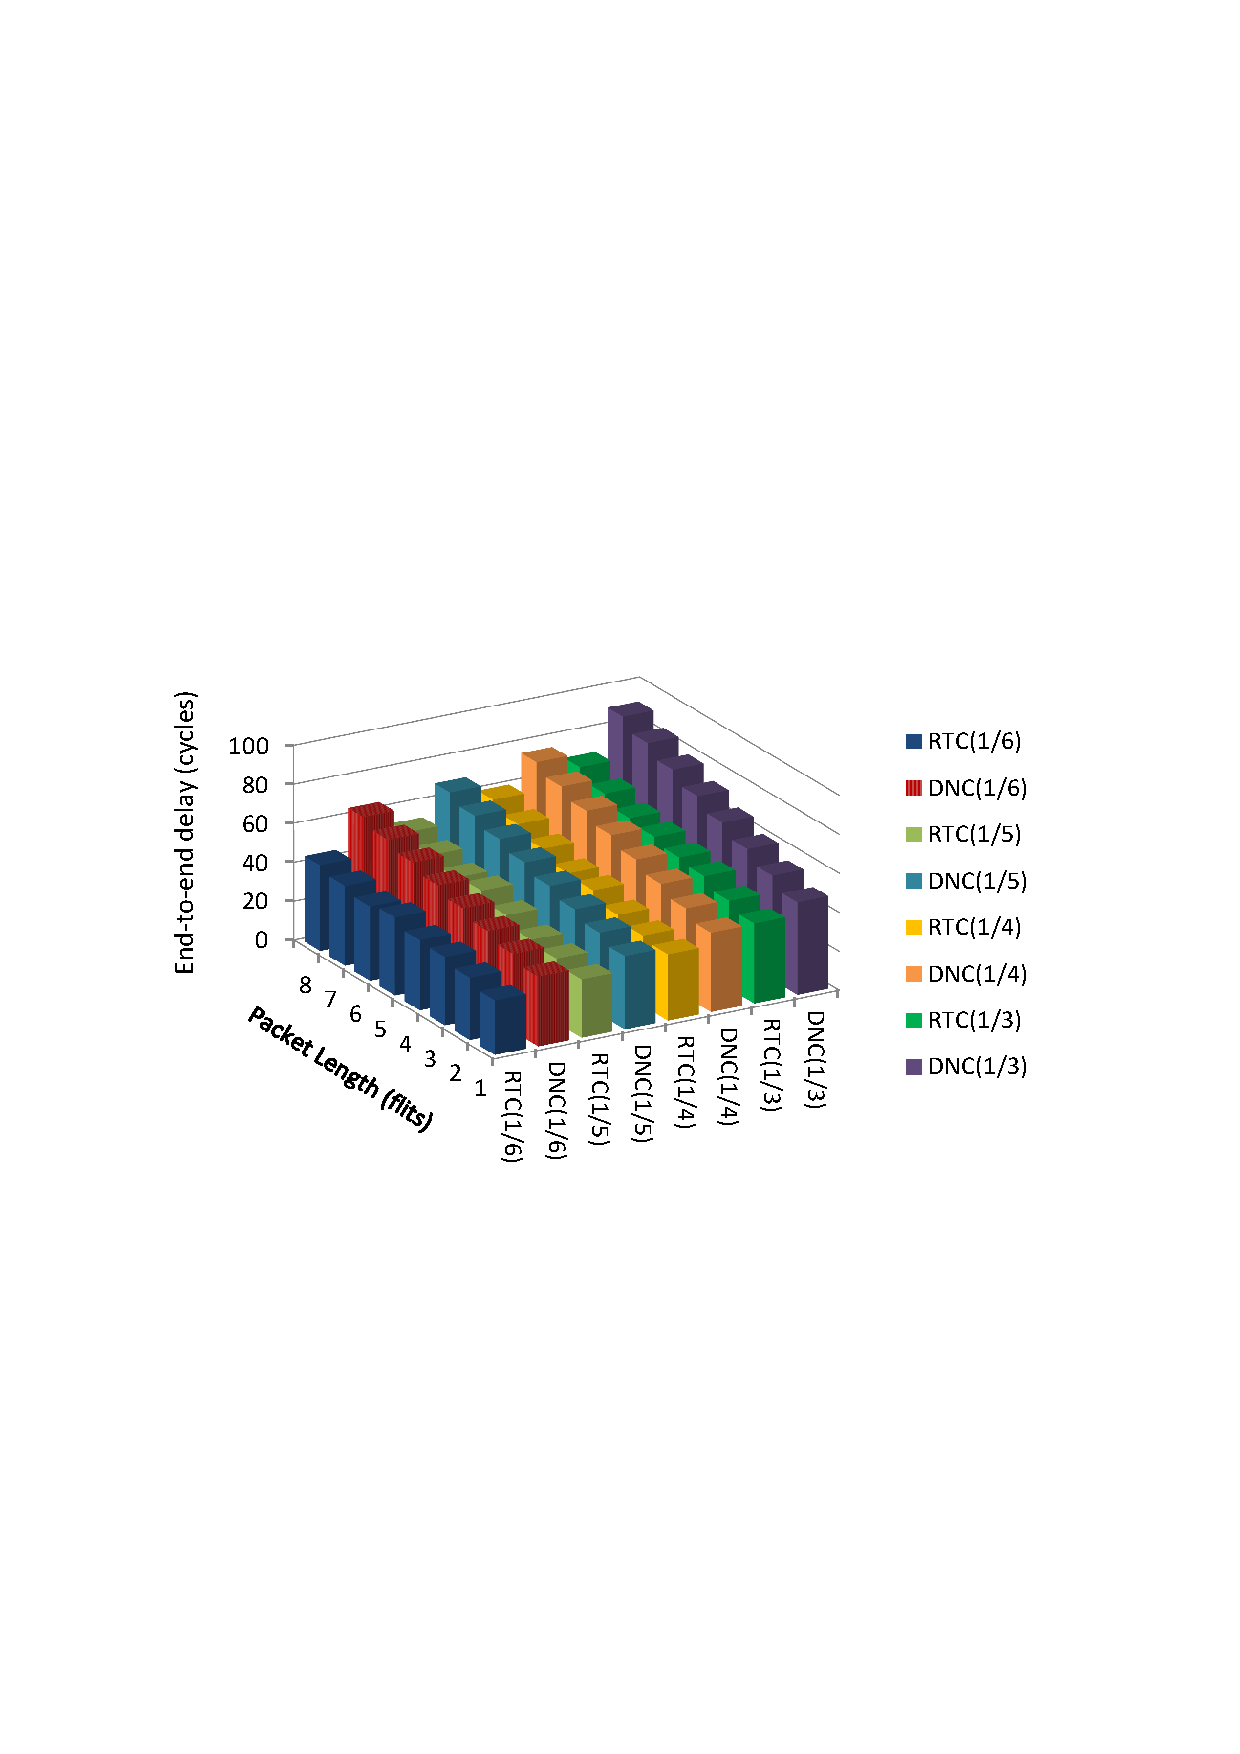
\includegraphics[scale=0.5]{fig12.pdf}\\
  \caption{Delay comparison with simulation under different packet length}\label{rtcvssim}
\end{figure}

For the errison application discussed in \cite{LuJa08}\cite{Jafari1922089}, we set the packet size to 128 bits, and collect the maximum end-to-end delay of each flow obtained by simulation. The comparison results between one simulation run and the delay bound calculated with our method are shown in Fig. \ref{ericsson}. The offset of each flow in this simulation run is zero cycle. We can see that the calculated delay bounds constrain the simulation results well, which verifies the correctness of our method. This comparison also demonstrates the ability of our method to analyze the real system with large number of flows.

\begin{figure*}
  \centering
  % Requires \usepackage{graphicx}
  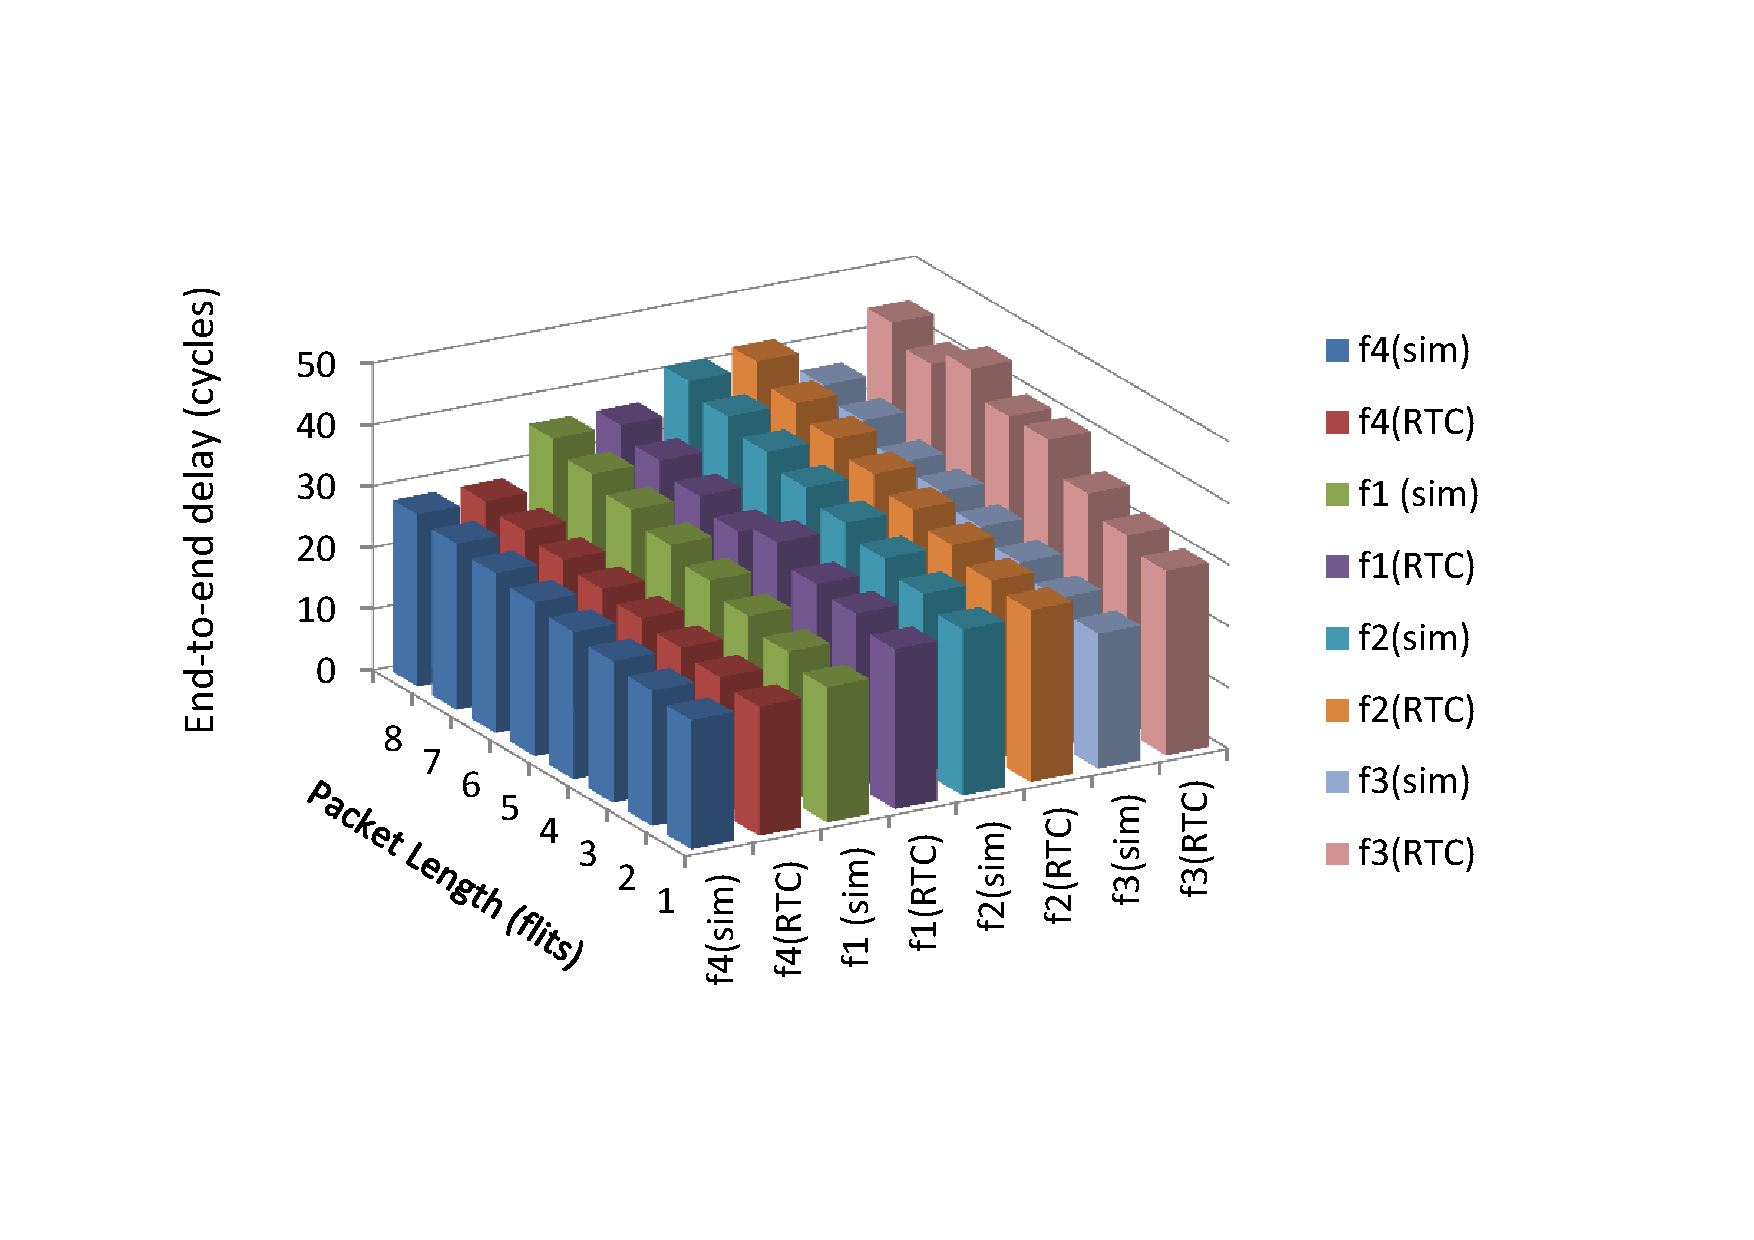
\includegraphics[scale=0.45]{fig13.pdf}\\
  \caption{Delay comparison with simulation}\label{ericsson}
\end{figure*}


\section{Conclusion}\label{conclusion}
The priority-aware wormhole-switched NoC is a promising platform for the on-chip real-time communication if the worst-case performance can be accurately analyzed and guaranteed. Simulation is not well suited for this purpose because it is difficult to cover all the corner cases. In this paper, we proposed an RTC-based performance model to achieve this goal. We first built the traffic model and service model for the priority-aware NoC, and then proposed a novel method to derive the upper service curve of credit-based flow control. Based on the proposed RTC model, we then proposed two end-to-end delay analysis algorithms and a buffer sizing algorithm. Our delay analysis algorithms can be implemented to compute the end-to-end delay for each flow automatically, and verify whether all these flows meet their deadline under the given configuration. Compared with the DNC-based performance model, our algorithms can give tighter delay bound since it takes the upper service curve and lower arrival curve into consideration. The proposed buffer sizing algorithm can optimize the buffer size from high-priority flows to low-priority flows. It can also be implemented to perform the buffer reduction automatically under the constraint of deadline. Compared with the LLBA method, our method can give much tighter buffer bound. Experimental results also illustrate that our method indeed outperforms the other analytical methods, e.g. LLBA and DNC, when the tightness of delay bound and buffer requirement are considered. Our method can be applied to the task mapping, routing and power reduction of priority-aware NoC.

\section*{Acknowledgements}
The authors thank the reviewers for their suggestions and comments, and all the experiments are carried out at the Integrated Microsystem Lab (IML) of McGill University. The first author also thank Ari Ramdial at McGill University for his helpful comments. This research is supported by High Technology
Research and Development Program of China (Grant No. 2012AA012201).

\bibliography{reference}


%%%%%%%%%%%%%%%%%%%%%%%%%%%%%%%%%%%%%%%%%%%%%%%%%%%%%%%%%%%%%%%%%%%%%%%%%%%%%%%%%%%%%%%%%%
%Author biography
%%%%%%%%%%%%%%%%%%%%%%%%%%%%%%%%%%%%%%%%%%%%%%%%%%%%%%%%%%%%%%%%%%%%%%%%%%%%%%%%%%%%%%%%%%
%\vspace{0.5in}
\parpic{\includegraphics[width=1in,height=1.25in,clip,keepaspectratio]{libl.pdf}}  \noindent{\bf Baoliang Li} was born in 1987. He received the B.S. degree in Computer Science and Technology from Tsinghua University, P.R. China, in 2009. He is currently working towards the Ph.D. degree from College of Computer at National University of Defense Technology (NUDT), P.R. China. His research interests is performance analysis of computer networks and Networks-on-Chip, with a special interest on the analytical methods of network calculus.

\vspace{0.1in}
\parpic{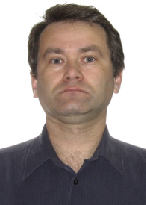
\includegraphics[width=1in,height=1.25in,clip,keepaspectratio]{zilic.pdf}}  \noindent{\bf Zeljko Zilic} received the B.Eng. degree from the University of Zagreb, Zagreb, Croatia, and the M.Sc. and Ph.D. degrees from the University of Toronto, Toronto, ON, Canada, all in electrical and computer engineering. He joined McGill University, Montreal, QC, Canada, in 1998, where he is currently an Associate Professor with the Department of Electrical and Computer Engineering. He conducts research on various aspects of the design and test of microsystems including programmable logic cores.

%\vspace{1.3in}
\parpic{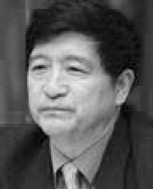
\includegraphics[width=1in,height=1.25in,clip,keepaspectratio]{douwh.pdf}} \noindent{\bf Wenhua Dou} was born in 1946. He received the B.S. degree in computer science from Harbin Military Engineering College in 1970. He has been working at National University of Defense Technology (NUDT), P.R. China since 1970. He was vice dean of College of Computer, NUDT from 1999 to 2003. He is currently a professor of College of Computer, NUDT with research focusing on computer networks.

\end{document}
